\begin{savequote}[75mm]
Q: What do you get when you cross a mosquito with a mountain climber?

A: Nothing. You can't cross a vector and a scalar.
%\qauthor{--- Queen Elizabeth II ---}
\end{savequote}

\chapter{Vector math}
\label{chap_vector}
\graphicspath{{figures/Vector/}}

For many applications, real numbers suffice, but are other times, these do not suffice.  Perhaps it is important to know, for instance, how close the nearest cuckoo's nest is as well as the direction in which it lies.  To answer questions like these which involve both a quantitative answer, or magnitude, along with a direction, we use the mathematical objects called \index{vector}\index[aut]{vector}\index{magnitude}\index[aut]{grootte}\index{direction}\index[aut]{richting}\textbf{vectors} (\textit{vector}).  


\section{Definition and representation}
\label{sec_vect_repre}
 A vector is represented geometrically as a directed line segment where the magnitude of the vector is taken to be the length of the line segment and the direction is made clear with the use of an arrow at one endpoint of the segment.  When referring to vectors in this text, we shall adopt the bold-faced arrow notation, so the symbol  $\vec{v}$ is read as the vector $v$.


In Figure~\ref{fig_vector_1a} is a typical vector $\vec{v}$ with endpoints $P\left(1, 2\right)$ and $Q\left(4, 6\right)$. The point $P$  is called the \index{vector ! initial point}\index[aut]{vector ! aangrijpingspunt}\textbf{initial point} or \index{vector ! tail}\textbf{head} (\textit{aangrijpingspunt}) of  $\vec{v}$ and the point $Q$ is called the \index{vector ! terminal point}\textbf{terminal point} or \index{vector ! head}\textbf{tail} of  $\vec{v}$.   Since we can reconstruct $\vec{v}$ completely from $P$ and $Q$, we write $\vec{v} = \overrightarrow{PQ}$, where the order of points $P$ (initial point) and $Q$ (terminal point) is important.

%\begin{figure}
%	\begin{center}
%		\includegraphics[width=0.35\textwidth]{fig_vector_1}
%		\caption{The vector $\vec{v} = \protect\overrightarrow{PQ}$. }
%		\label{fig_vector_1}
%	\end{center}
%\end{figure}

While it is true that $P$ and $Q$ completely determine $\vec{v}$, it is important to note that since vectors are defined in terms of their two characteristics,  \index{vector ! magnitude}\index[aut]{vector ! grootte}\textbf{magnitude} (\textit{grootte}) and \index{vector ! direction}\index[aut]{vector ! richting}\textbf{direction} (\textit{richting}), any directed line segment with the same length and direction as $\vec{v}$ is considered to be the same vector as $\vec{v}$, regardless of its initial point. In the case of our vector $\vec{v}$ above, any vector which moves three units to the right and four up from its initial point to arrive at its terminal point is considered the same vector as $\vec{v}$.  The notation we use to capture this idea is the \index{vector ! component form}\textbf{component form} of the vector, $\vec{v} = \left(3,4\right)$, where the first number, $3$, is called the \textbf{$\boldsymbol{x}$-component} (\textit{$x$-component}) of $\vec{v}$ and the second number, $4$, is called the \index{vector ! component form}\textbf{$\boldsymbol{y}$-component} (\textit{$y$-component}) of $\vec{v}$.  If we wanted to reconstruct $\vec{v} = \left(3,4\right)$ with initial point $\widetilde{P}(-2,3)$, then we would find the terminal point of $\vec{v}$ by adding $3$ to the $x$-coordinate and adding $4$ to the $y$-coordinate to obtain the terminal point $\widetilde{Q}(1,7)$ (Figure~\ref{fig_vector_2}).

%\begin{figure}
%	\begin{center}
%		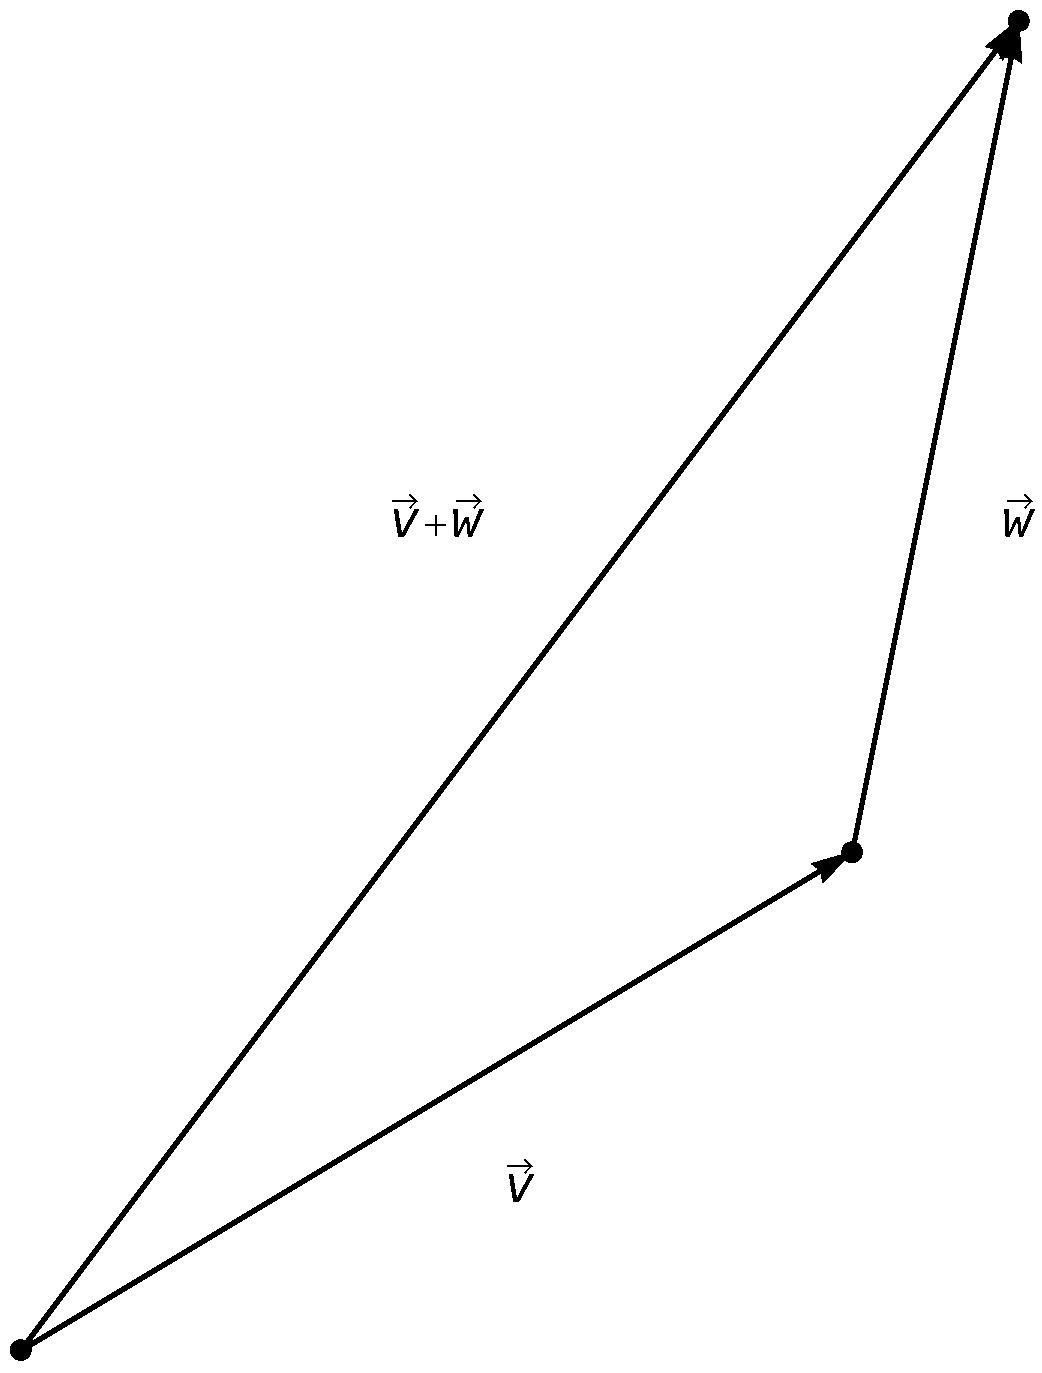
\includegraphics[width=0.35\textwidth]{fig_vector_2}
%		\caption{$\vec{v} = \left(3,4\right)$ with initial point $\widetilde{P}(-2,3)$. }
%		\label{fig_vector_2}
%	\end{center}
%\end{figure}

\begin{figure}[H]
\centerline{
\subfigure[\label{fig_vector_1a}]{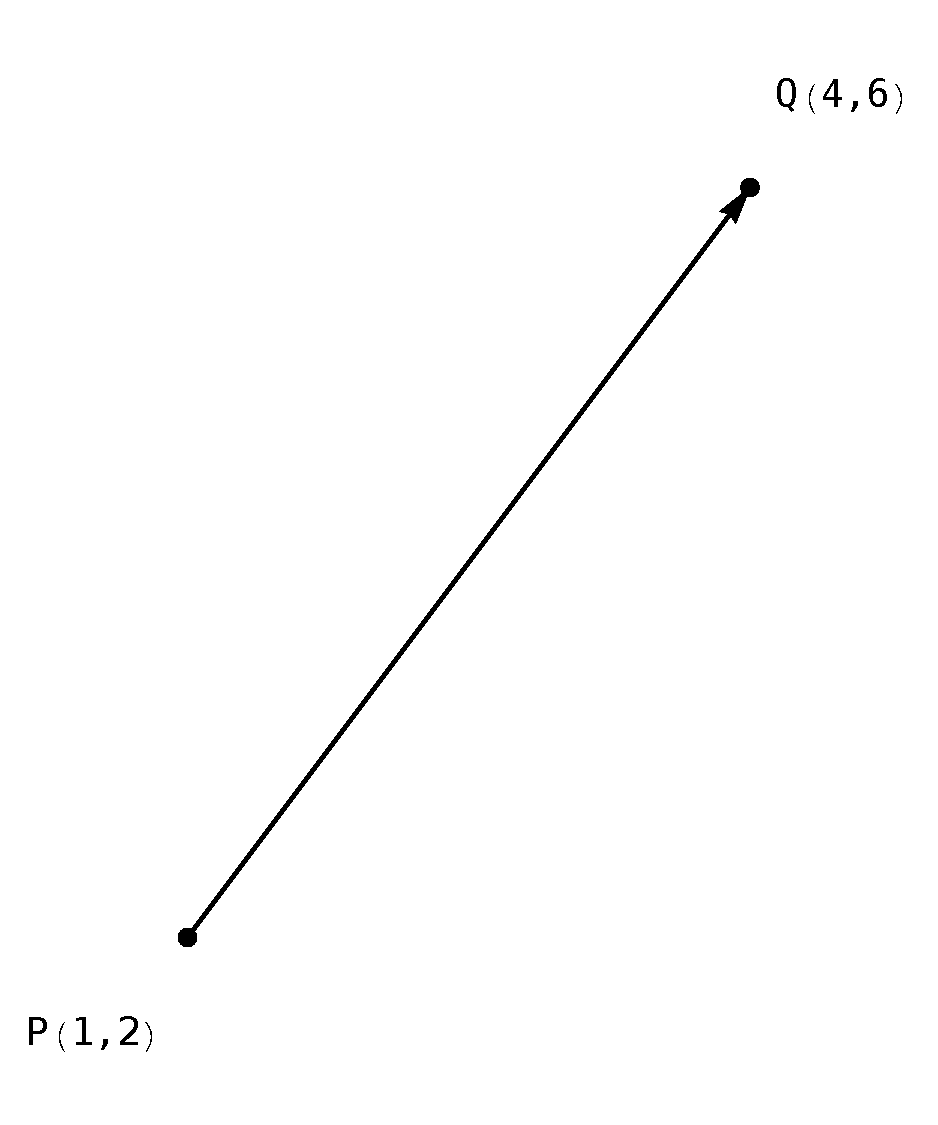
\includegraphics[width=0.35\textwidth]{fig_vector_1a}}
\hspace{0.1cm}
\subfigure[\label{fig_vector_1b}]{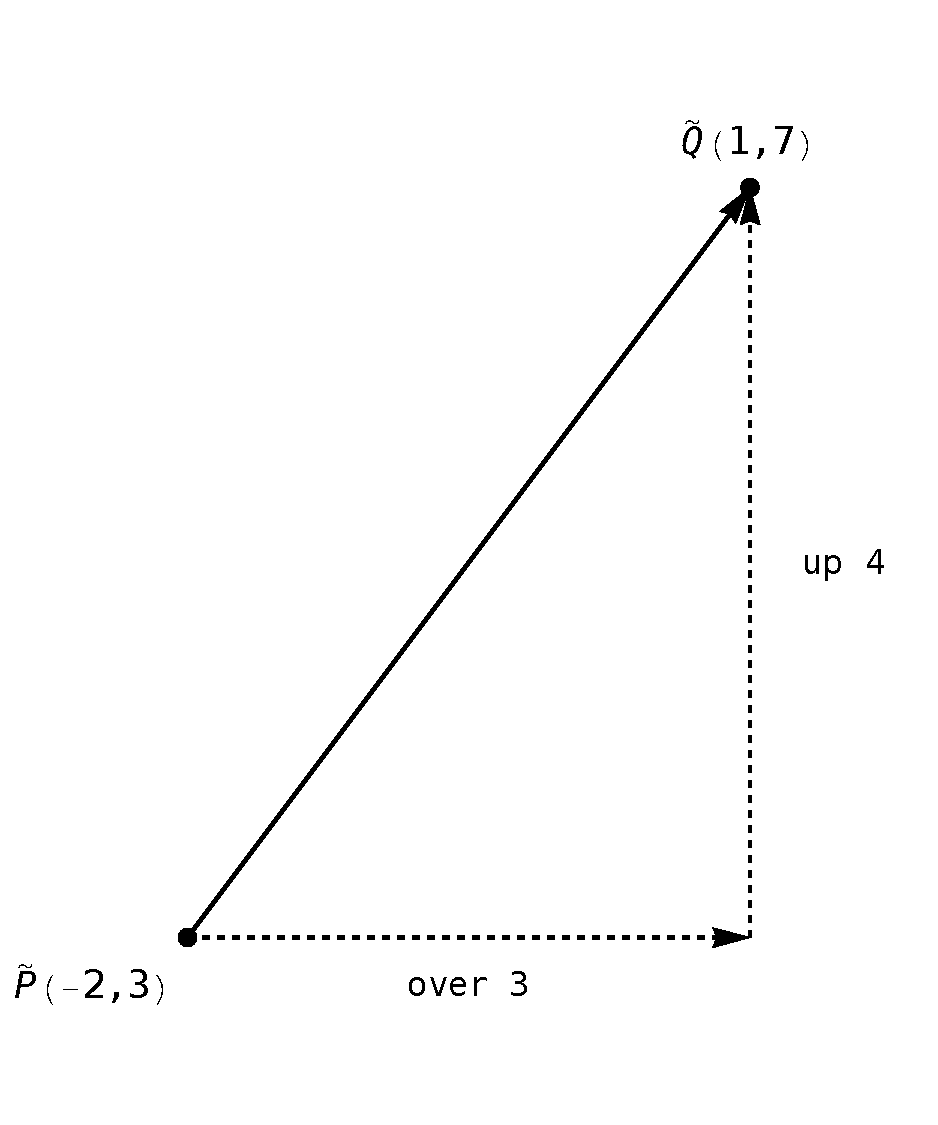
\includegraphics[width=0.35\textwidth]{fig_vector_1b}}
}
\caption{ $\vec{v} = \left(3,4\right)$ with initial point $P(1,2)$ (a) and $\widetilde{P}(-2,3)$ (b).}
\end{figure}

This idea is formalized in the following definition. 

\begin{definition}[Component form of a vector] \label{componentformvector}  Suppose $\vec{v}$ is represented by a directed line segment with initial point $P\left(x_0, y_0\right)$ and terminal point $Q\left(x_1, y_1\right)$.  The component form of $\vec{v}$ is given by 

\[ \vec{v} = \overrightarrow{PQ} = \left( x_1 - x_0, y_1 - y_0 \right). \]


\end{definition}

Using the language of components, we have that two vectors are equal if and only if their corresponding components are equal.  That is, $\left(v_1, v_2\right) = \left(\widetilde{v}_1, \widetilde{v}_2\right)$ if and only if $v_1 = \widetilde{v}_1$ and $v_2 = \widetilde{v}_2$. 


\section{Vector arithmetic}
\label{sec_vector_arith}
\subsection{Addition}
We are now set to define operations on vectors.  Suppose we are given two vectors $\vec{v}$ and $\vec{w}$.  The sum $\vec{v} + \vec{w}$ is obtained as illustrated in Figure~\ref{fig_vector_2}.  First, plot $\vec{v}$.  Next, plot $\vec{w}$ so that its initial point is the terminal point of $\vec{v}$.  To plot the vector $\vec{v} + \vec{w}$ we begin at the initial point of $\vec{v}$ and end at the terminal point of $\vec{w}$.  It is helpful to think of the vector $\vec{v} + \vec{w}$ as the net result of moving along $\vec{v}$ then moving along $\vec{w}$. 

\begin{figure}
	\begin{center}
			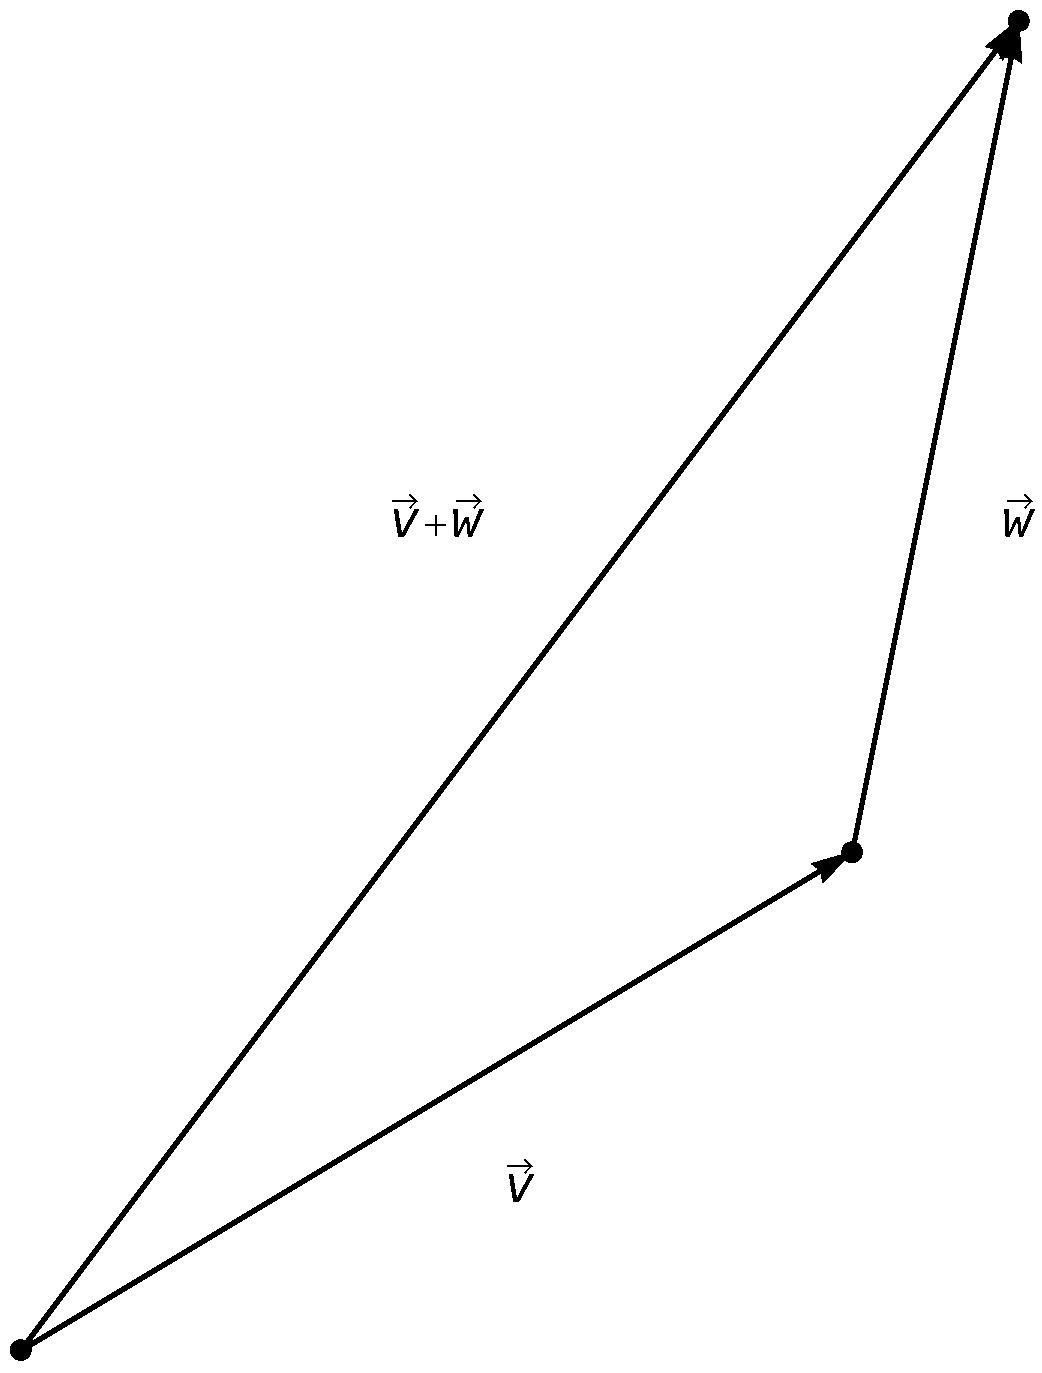
\includegraphics[width=0.25\textwidth]{fig_vector_2}
	\caption{The vectors $\vec{v}$ and $\vec{w}$ and their sum $\vec{v}+\vec{w}$. }
	\label{fig_vector_2}
	\end{center}
\end{figure}

\begin{example} \label{vectorbearingex}  
A plane leaves an airport with an airspeed  of 175 kilometres per hour at a  bearing of  N$40^{\circ}$E.  A 35 kilometres per hour wind is blowing at a bearing of S$60^{\circ}$E.  Find the speed and  bearing of the plane.

\xhrulefill{gray}{2.5pt}Solution \xhrulefill{gray}{2.5pt}

For both the plane and the wind, we are given their speeds and their directions.  Coupling speed (as a magnitude) with direction is the concept of velocity. We let $\vec{v}$ denote the plane's velocity and $\vec{w}$ denote the wind's velocity in the diagram below.   The true speed and bearing is found by analysing the vector $\vec{v} + \vec{w}$ (Figure~\ref{fig_vector_3a}).  From the vector diagram, we get a triangle, the lengths of whose sides are the magnitude of $\vec{v}$, which is 175, the magnitude of $\vec{w}$, which is 35, and the magnitude of $\vec{v} + \vec{w}$, which we call $c$ (Figure~\ref{fig_vector_3b}). From the given bearing information, we go through the usual geometry to determine that the angle between the sides of length 35 and 175 measures $100^{\circ}$. 

From the law of cosines, we determine $c = \sqrt{31850 - 12250\cos(100^{\circ})} \approx 184$, which means the true speed of the plane is (approximately) $184$ kilometres per hour.  To determine the true bearing of the plane, we need to determine the angle $\alpha$.  Using the law of cosines once more, we find $\cos(\alpha) = \frac{c^2+29400}{350c}$ so that $\alpha \approx 11^{\circ}$.  Given the geometry of the situation, we add $\alpha$ to the given $40^{\circ}$ and find the true bearing of the plane to be (approximately) N$51^{\circ}$E. 

\begin{figure}[H]
\centering
%\right)isebox{0.5cm}{
\centerline{
\subfigure[\label{fig_vector_3a}]{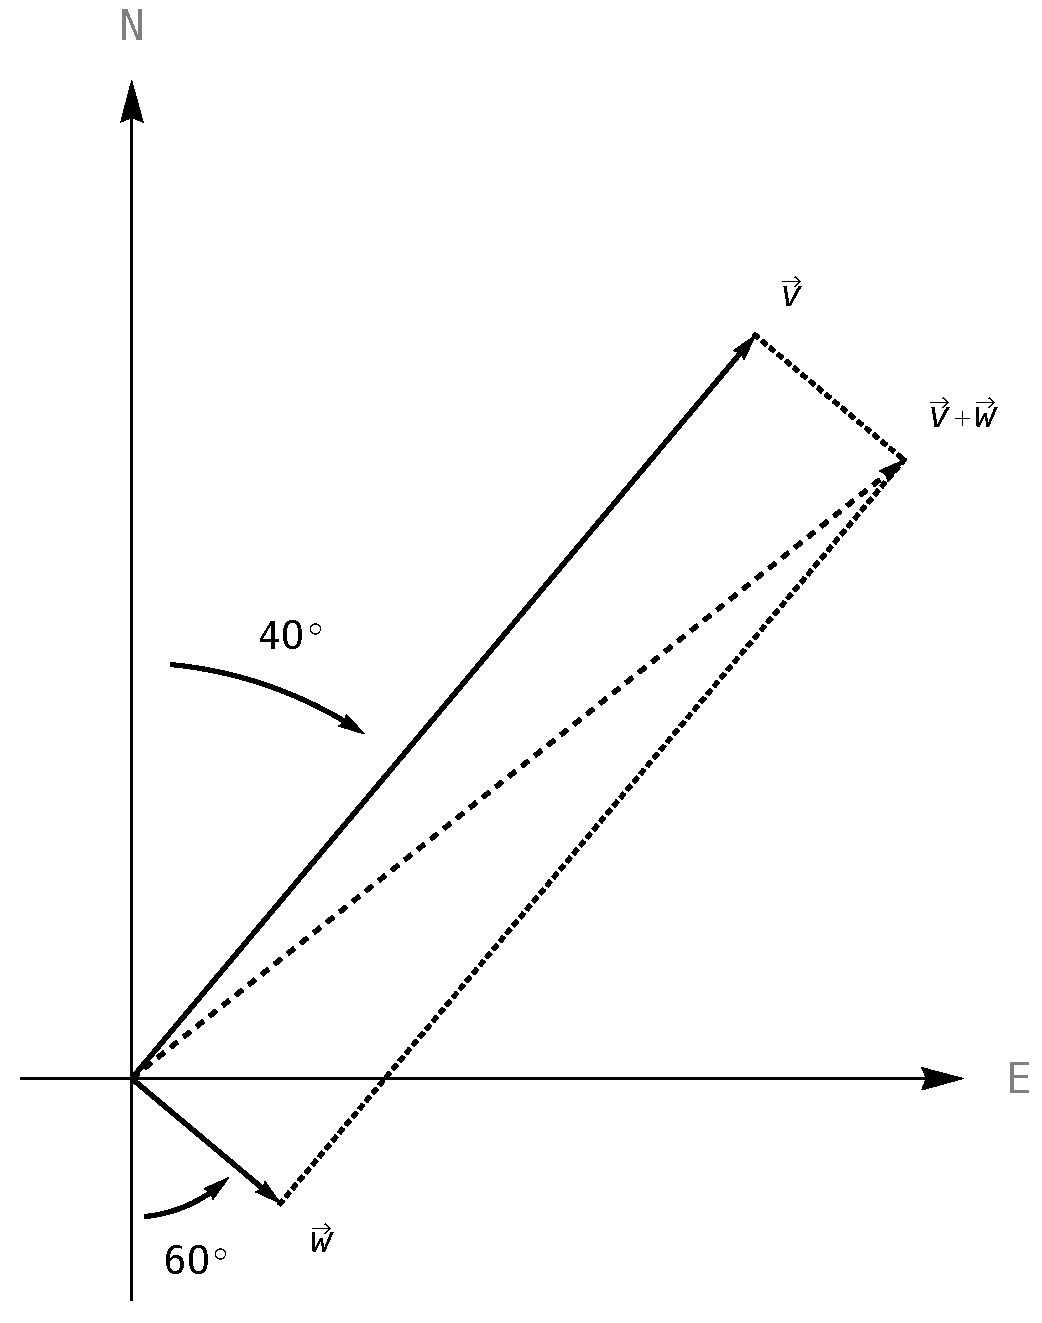
\includegraphics[width=0.4\textwidth]{fig_vector_3a}}
\hspace{0.1cm}
\subfigure[\label{fig_vector_3b}]{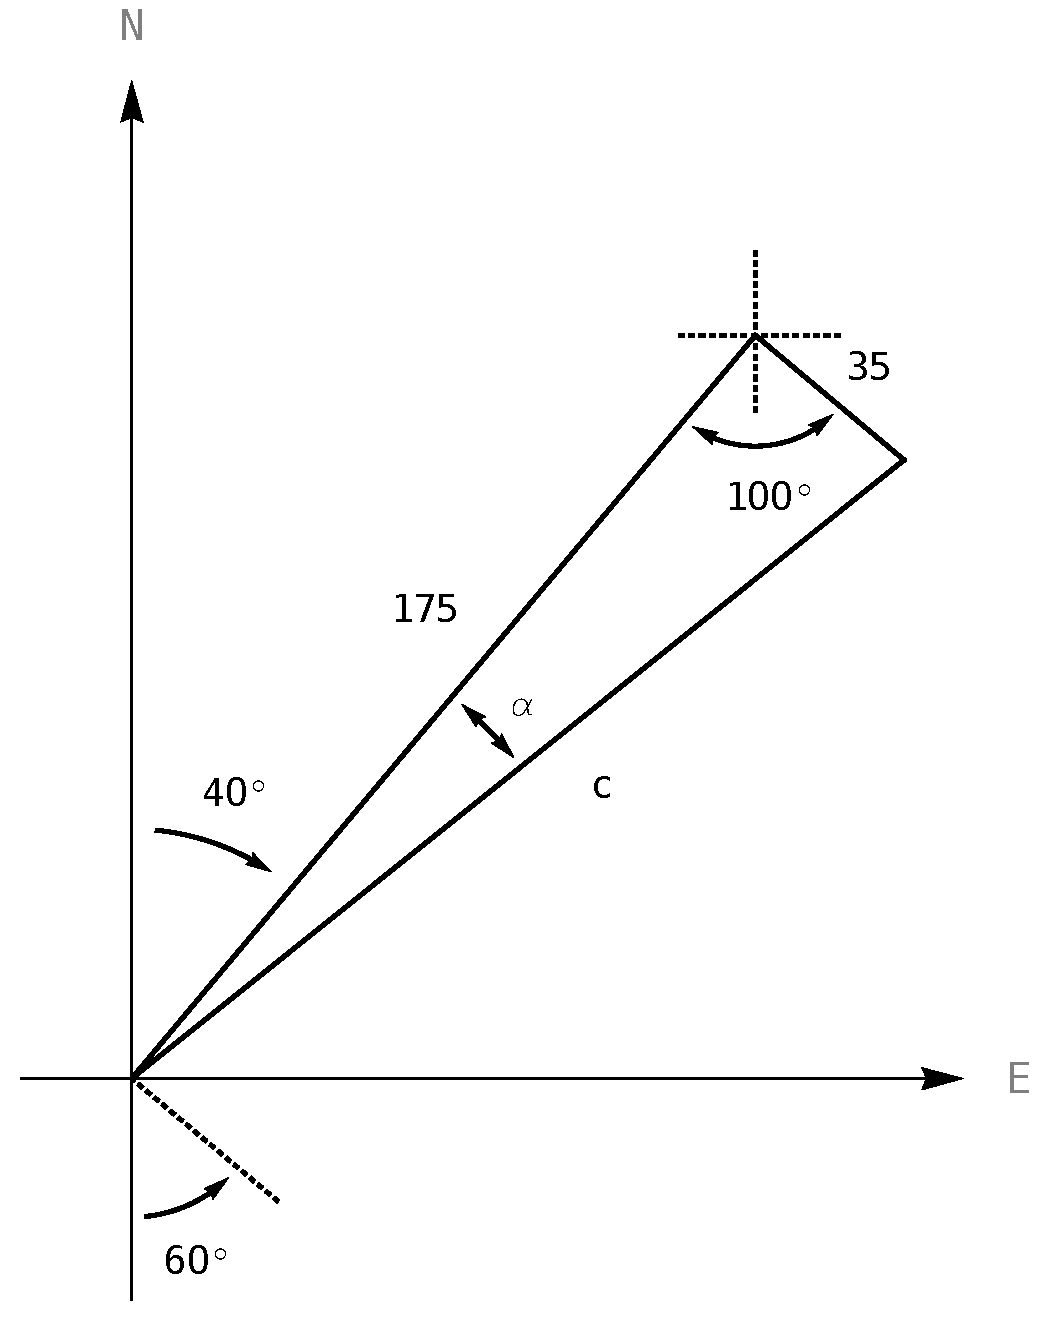
\includegraphics[width=0.4\textwidth]{fig_vector_3b}}
}
\caption{Finding the speed and bearing of a plane travelling at 175 kilometres per hour at a  bearing of  N$40^{\circ}$E under a 35 kilometre per hour wind is blowing at a bearing of S$60^{\circ}$E. }

\end{figure}


\end{example}

Having now a geometric understanding of the addition of vectors, we are ready to give its algebraic counterpart.

\begin{definition}[Vector addition] \label{vectoradd} 
 Suppose $\vec{v} = \left(v_1,v_2\right)$ and $\vec{w} = \left(w_1,w_2\right)$.  The vector $\vec{v} + \vec{w}$ is defined by \index{vector ! addition}\index[aut]{vector ! som}

\[ \vec{v} + \vec{w}  = \left( v_1 + w_1, v_2 + w_2 \right). \]


\end{definition}


In order for vector addition to enjoy the same kinds of properties as real number addition, it is necessary to extend our definition of vectors to include a \textbf{zero vector} (\textit{nulvector}) \index{zero vector)} \index[aut]{nulvector}, $\vec{0} = \left(0, 0\right)$.  Geometrically,  $\vec{0}$ represents a point, which we can think of as a directed line segment with the same initial and terminal points. The direction of $\vec{0}$ is in fact undefined. Having introduced the vector counterpart of the real number 0, we can go ahead and list the properties of vector addition, which are completely in line with those for real numbers. Essentially, for all vectors $\vec{v} \text{ and } \vec{w}$ we have

\index{commutativity}\index[aut]{commutativiteit}\index{associativity}\index[aut]{associativiteit}\index{neutral element}\index[aut]{neutraal element}\index{inverse element}\index[aut]{invers element}

\begin{itemize}

\item  \textbf{Commutative property:}  
$$\vec{v} + \vec{w} = \vec{w} + \vec{v}\,,$$

\item  \textbf{Associative property:}  
$$\left(\vec{u} + \vec{v}\right) + \vec{w} = \vec{u} + \left(\vec{v} + \vec{w}\right)\,,$$

\item  \textbf{Identity property:} 
 \[\vec{v} + \vec{0} = \vec{0} + \vec{v} = \vec{v}\,,\] 

\item  \textbf{Inverse property:} for every vector $\vec{v}$, there is a vector $-\vec{v}$ so that \[\vec{v} + (-\vec{v}) = (-\vec{v}) + \vec{v} = \vec{0}.\] 

\end{itemize}

\ifanalysis
\begin{proof}
These properties are easily verified using the definition of vector addition. For instance, for the commutative property, we note that if $\vec{v} = \left(v_1,v_2\right)$ and $\vec{w} = \left(w_1,w_2\right)$ then

\[ \begin{array}{rcl} \vec{v} + \vec{w}  & = &  \left( v_1, v_2 \right) +  \left(  w_1, w_2 \right) \\
& = & \left( v_1 + w_1, v_2 + w_2 \right) \\
& = &  \left( w_1 + v_1, w_2 + v_2 \right) \\
& = & \vec{w} + \vec{v}. \end{array} \]


Geometrically, we can see the commutative property by realizing that the sums $\vec{v}+\vec{w}$ and $\vec{w} + \vec{v}$ are the same directed diagonal determined by the parallelogram in Figure~\ref{fig_vector_4}. The proofs of the associative and identity properties proceed similarly. 
\end{proof}
\fi

\begin{figure}
	\begin{center}
			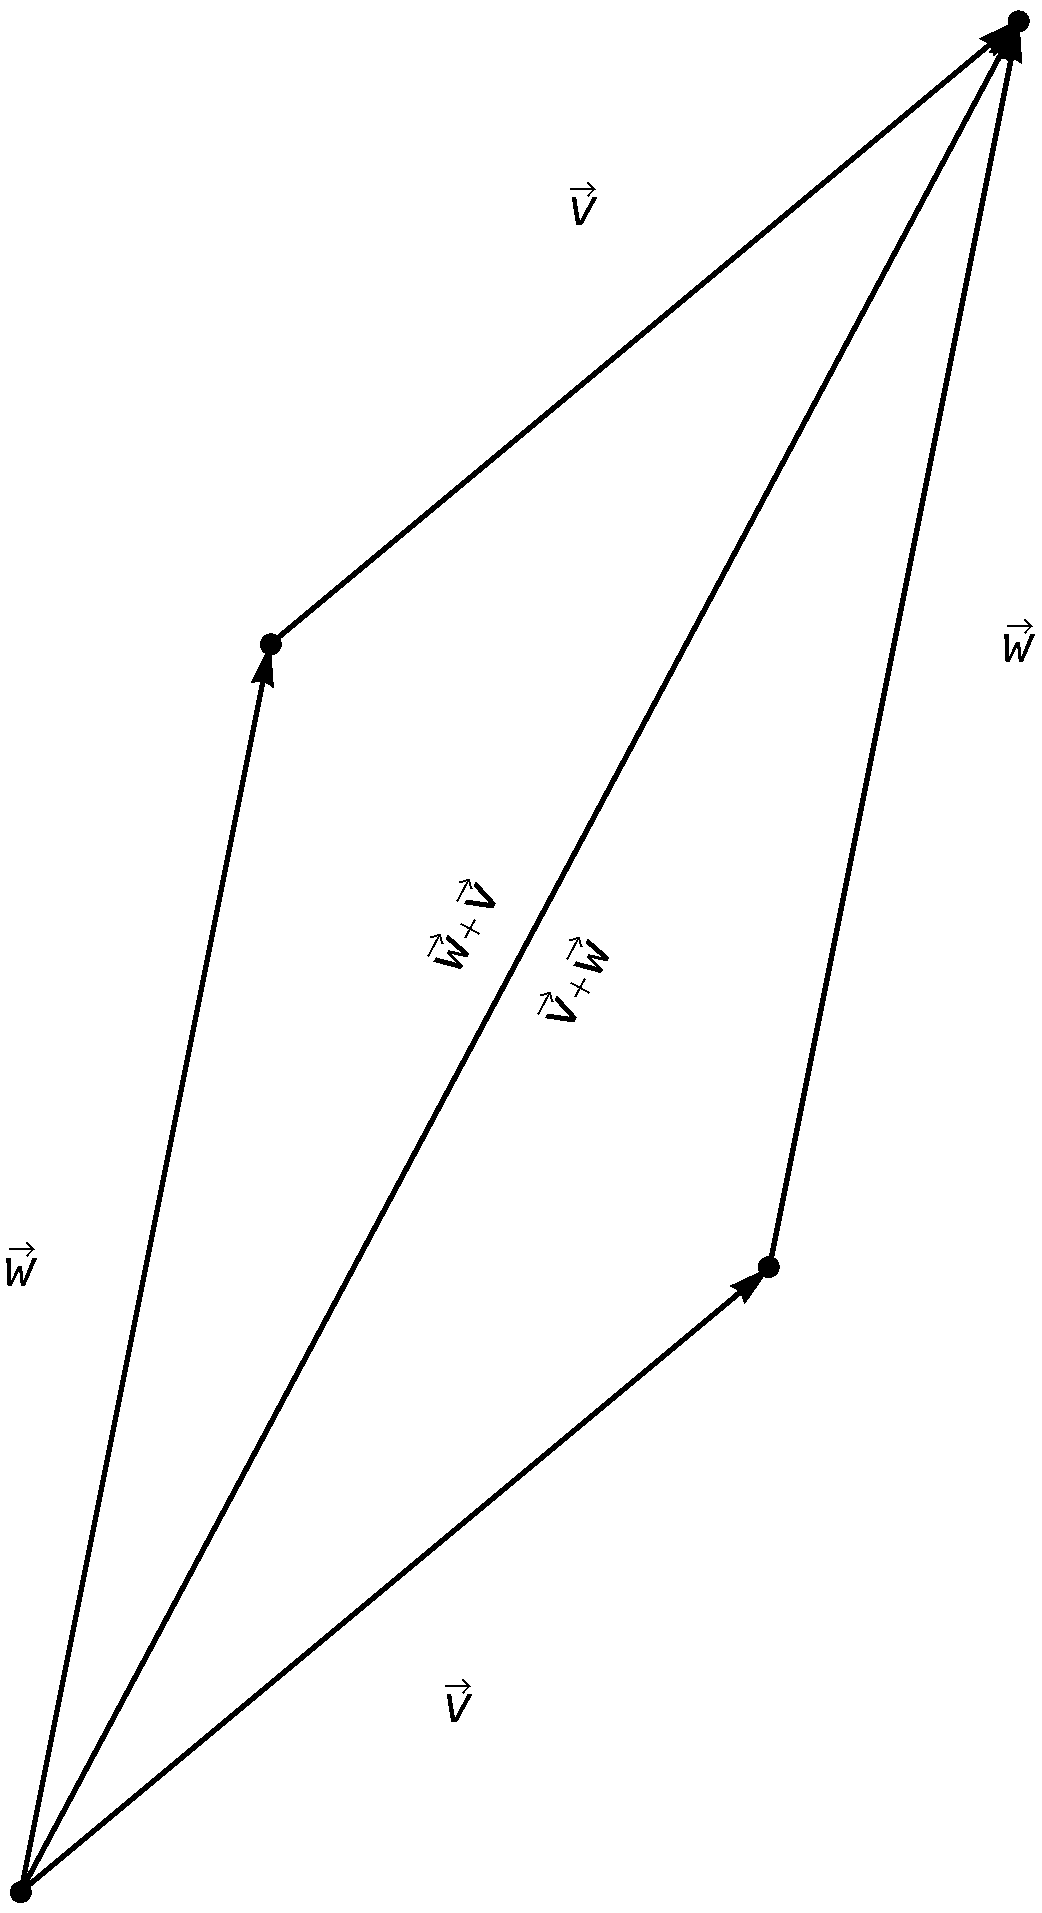
\includegraphics[width=0.25\textwidth]{fig_vector_4}
	\caption{Proving the commutative property of vector addition. }
	\label{fig_vector_4}
	\end{center}
\end{figure}

For what concerns the additive inverse $-\vec{v} = \left(-v_1, -v_2\right)$  of a vector $\vec{v} = \left(v_1, v_2\right)$, it is clear that both vectors have the same length, but opposite directions.  As a result, when adding the vectors geometrically, the sum $\vec{v} + (-\vec{v})$ results in starting at the initial point of $\vec{v}$ and ending back at the initial point of $\vec{v}$, or in other words, the net result of moving $\vec{v}$ then $-\vec{v}$ is not moving at all.  Using the additive inverse of a vector, we can define the difference of two vectors, $\vec{v} - \vec{w} = \vec{v} + (-\vec{w})$.   If $\vec{v} = \left(v_1,v_2\right)$ and $\vec{w} = \left(w_1,w_2\right)$ then  

\[\begin{array}{rcl} \vec{v} - \vec{w} & = & \vec{v} + (-\vec{w}) \\
&  = & \left(v_1,v_2\right) + \left(-w_1,-w_2\right) \\
& = &  \left(v_1 + \left(-w_1\right),v_2 + \left(-w_2\right) \right)\\
& = &  \left(v_1 -w_1,v_2 - w_2\right). \\ \end{array} \]

In other words, like vector addition, vector subtraction works component-wise.   From the diagram in Figure~\ref{fig_vector_5}, we see that  $\vec{v}-\vec{w}$ may be interpreted as the vector whose initial point is the terminal point of $\vec{w}$ and whose terminal point is the terminal point of $\vec{v}$ as depicted below.  It is also worth mentioning that in the parallelogram determined by the vectors $\vec{v}$ and $\vec{w}$, the vector $\vec{v}-\vec{w}$ is one of the diagonals -- the other being $\vec{v} + \vec{w}$.

\begin{figure}[h]
	\begin{center}
			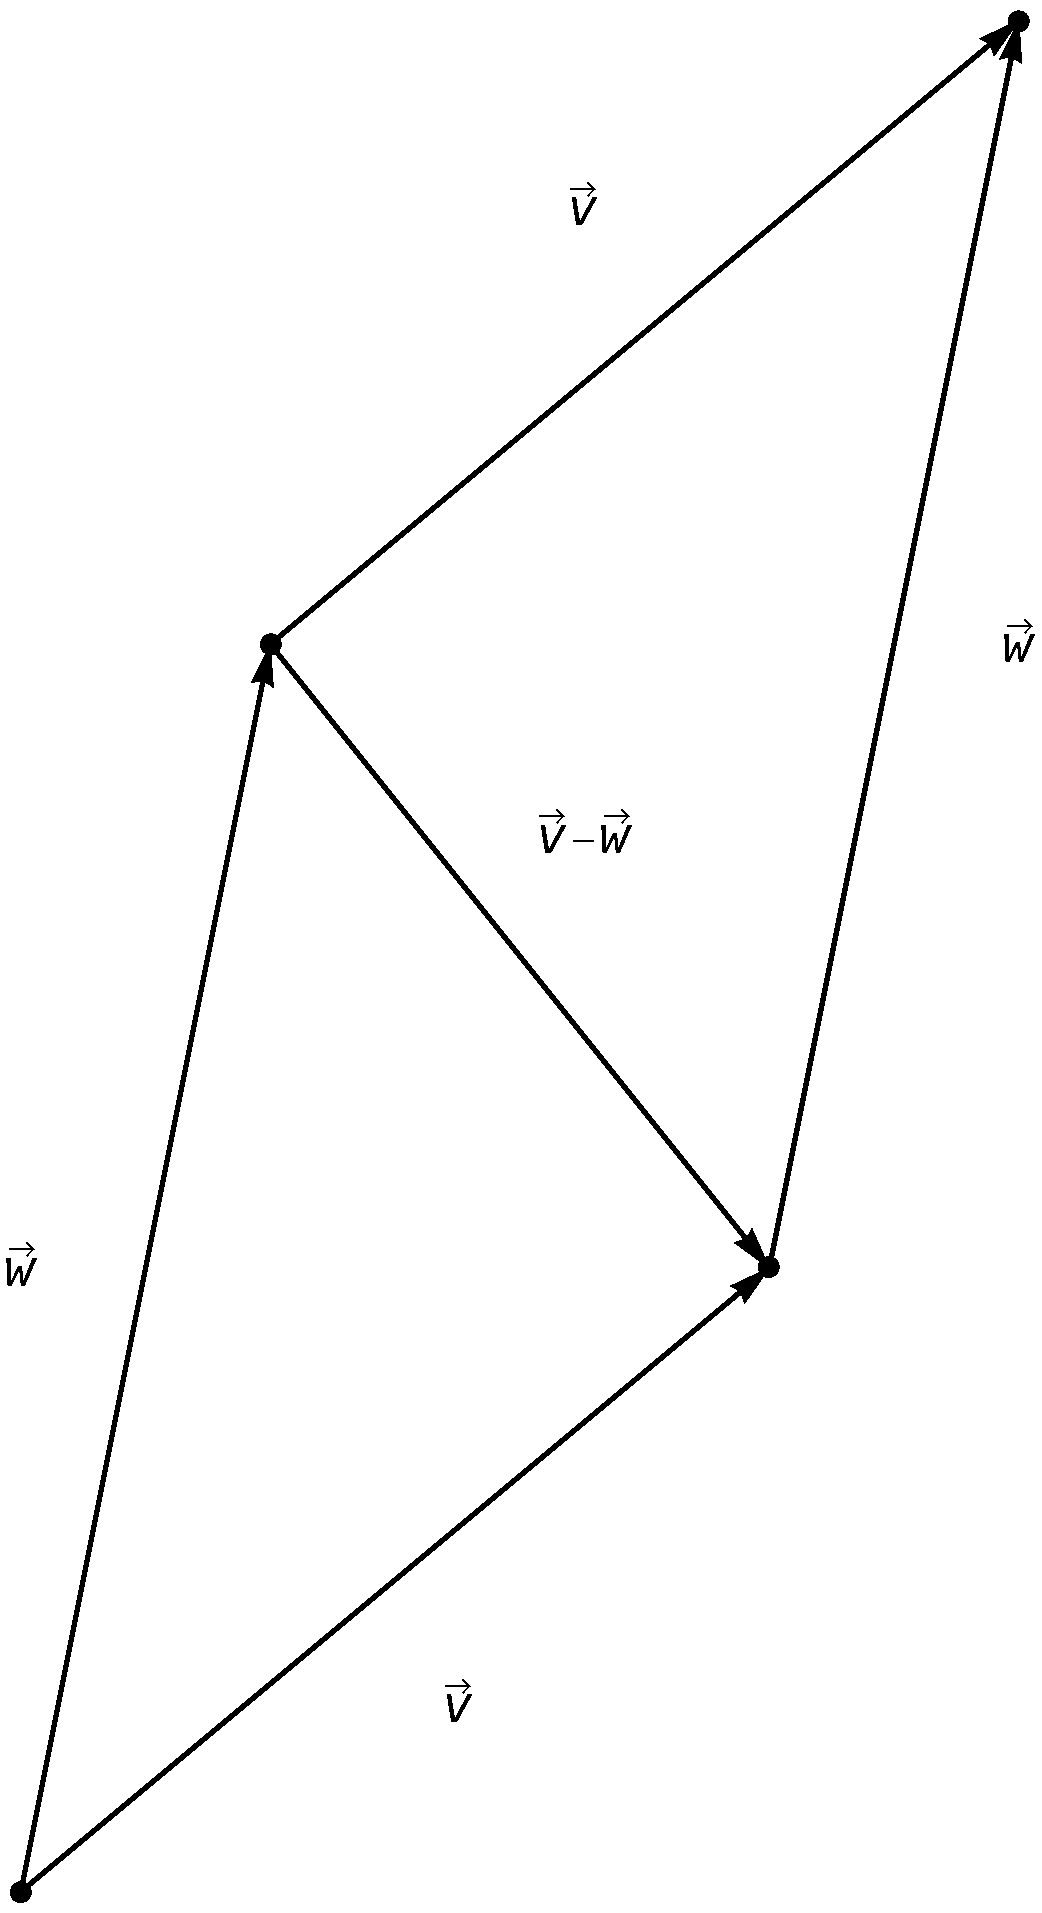
\includegraphics[width=0.25\textwidth]{fig_vector_5}
	\caption{The vectors $\vec{v}$ and $\vec{w}$ and their difference $\vec{v}-\vec{w}$. }
	\label{fig_vector_5}
	\end{center}
\end{figure}

\ifcalculus
\begin{example}  \label{vectoraddex} 
 Let  $\vec{v} = \left(3,4\right)$ and suppose  $\vec{w} = \overrightarrow{PQ}$ where $P(-3,7)$ and $Q(-2,5)$.  Find $\vec{v} + \vec{w}$ and interpret this sum geometrically.


\xhrulefill{gray}{2.5pt}Solution \xhrulefill{gray}{2.5pt}


First, we need to write  $\vec{w}$ in component form, which yields $\vec{w} = \left(-2-(-3),5-7\right) = \left(1,-2\right)$.  Thus $\vec{v} + \vec{w}  =   \left(3,4\right) + \left(1,-2\right)=\left( 3 + 1, 4 + (-2) \right)=\left(4, 2\right).$


                                        
To visualize this sum in Figure~\ref{fig_vector_6}, we draw $\vec{v}$ with its initial point at $(0,0)$ for convenience so that its terminal point is $(3,4)$.  Next, we graph $\vec{w}$ with its initial point at $(3,4)$.  Moving one to the right and two down, we find the terminal point of $\vec{w}$ to be $(4,2)$.  We see that the vector $\vec{v} + \vec{w}$ has initial point $(0,0)$ and terminal point $(4,2)$ so its component form  is $\left(4,2\right)$, as required.

\begin{figure}[H]
	\begin{center}
			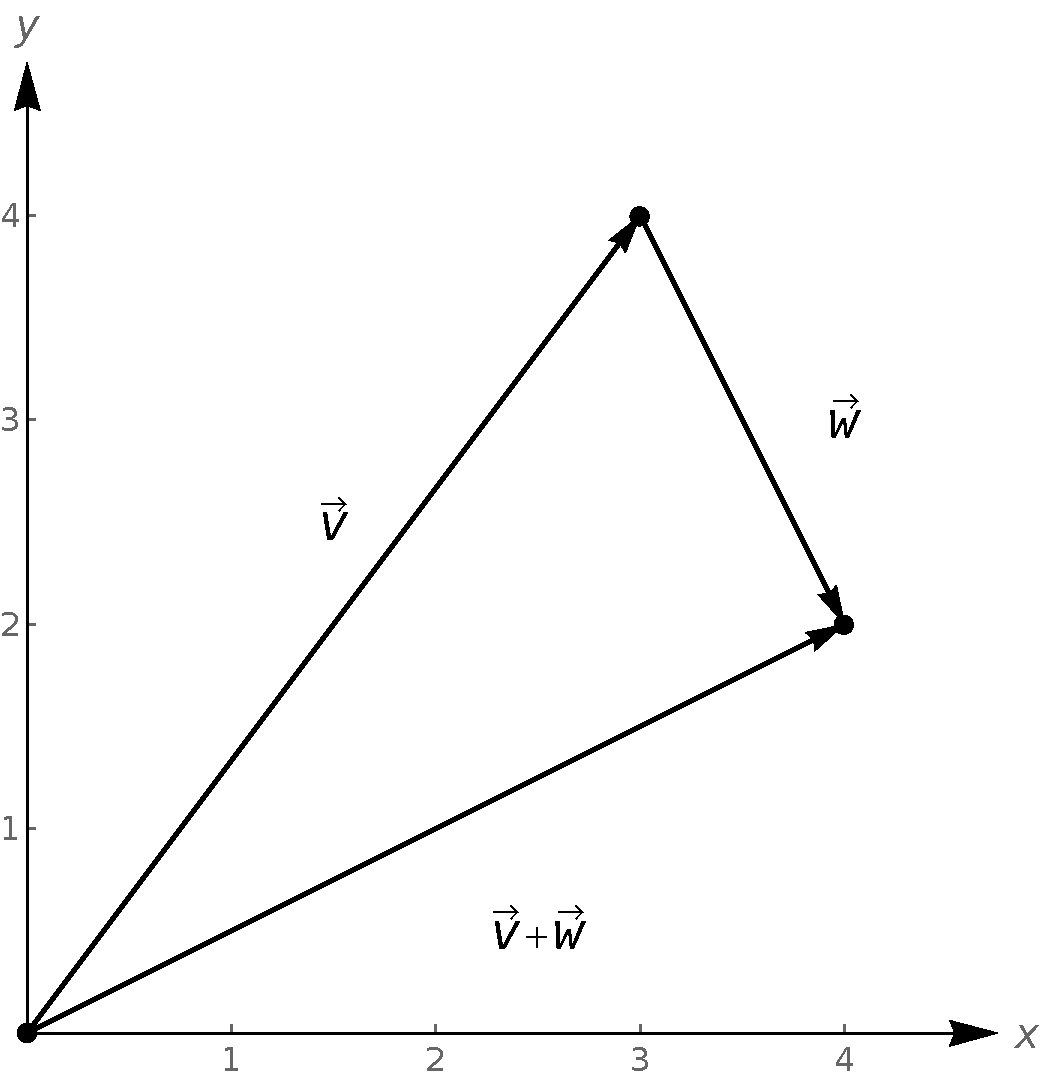
\includegraphics[width=0.35\textwidth]{fig_vector_6}
	\caption{The vectors $\vec{v} = \left(3,4\right)$  and $\vec{w}=\left(1,-2\right)$ and their sum. }
	\label{fig_vector_6}
	\end{center}
\end{figure}


\end{example}
\fi

\subsection{Scalar multiplication}

Next, we discuss \textbf{scalar multiplication} (\textit{scalaire vermenigvuldiging}) -- that is, taking a real number times a vector.  


\begin{definition}[Scalar multiplication] \label{scalarmultvector} \index{vector ! scalar multiplication} \index{scalar multiplication}\index[aut]{vector ! scalaire vermenigvuldiging} \index[aut]{scalaire vermenigvuldiging} If $k$ is a real number and $\vec{v} = \left(v_1,v_2\right)$, we define $k\vec{v}$ by 
\[k\vec{v} = k\left(v_1,v_2\right) =\left(k v_1,k v_2\right). \]

\end{definition}

Scalar multiplication by $k$ in vectors can be understood geometrically as scaling the vector (if $k > 0$) or scaling the vector and reversing its direction (if $k < 0$) as demonstrated in Figure~\ref{fig_vector_7}.

\begin{figure}
	\begin{center}
			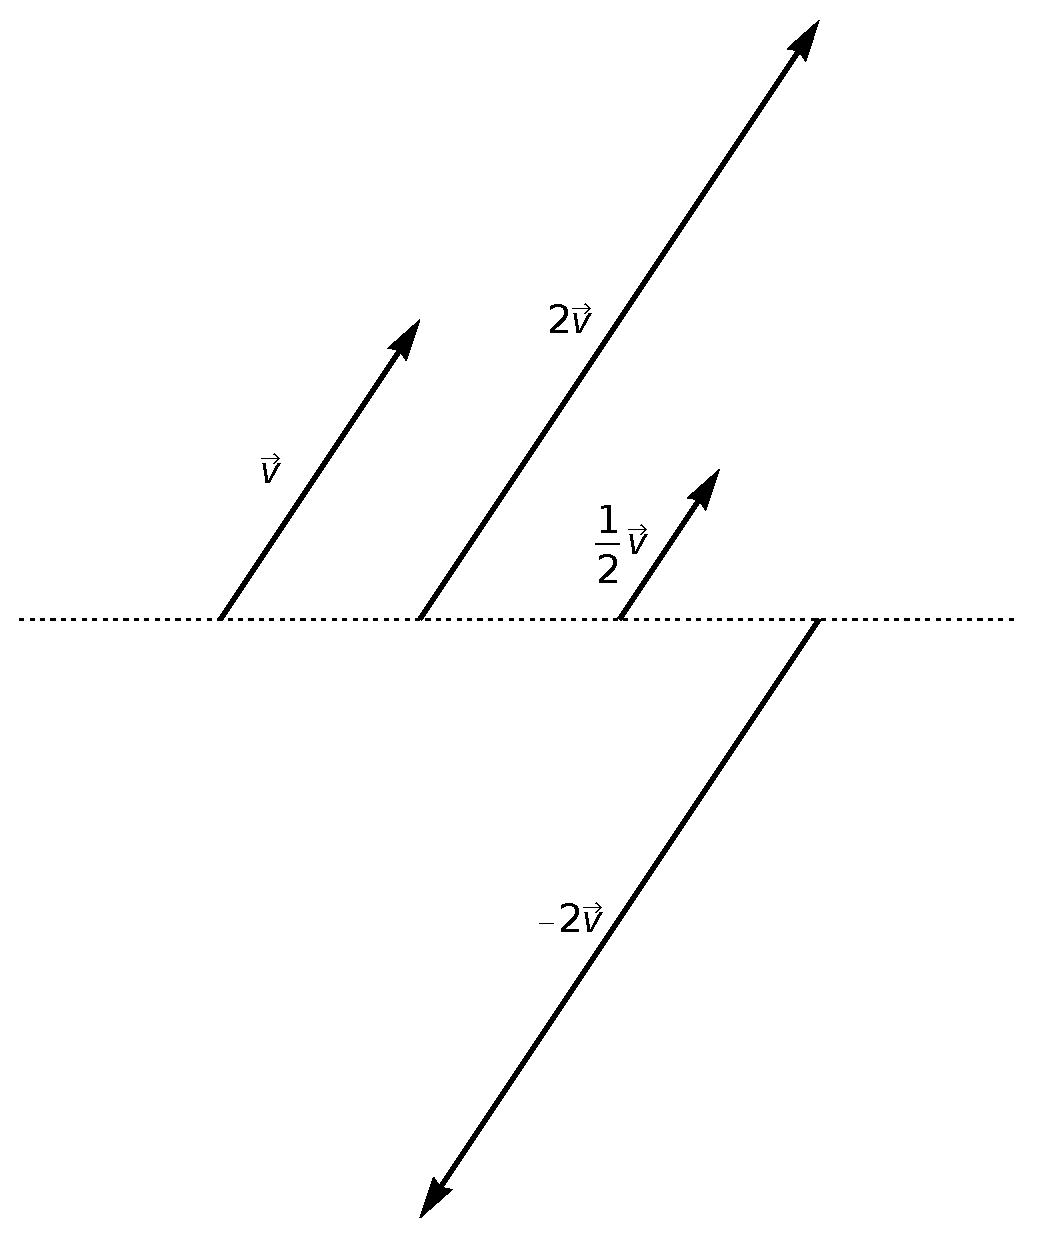
\includegraphics[width=0.35\textwidth]{fig_vector_7}
	\caption{The scalar multiplication of a vector $\vec{v}$. }
	\label{fig_vector_7}
	\end{center}
\end{figure}

 The properties of scalar multiplication are summarized below for vectors $\vec{v}$ and $\vec{w}$ and scalars  $k$ and $r$.

\index{distributivity}\index[aut]{distributiviteit}\index{associativity}\index[aut]{associativiteit}\index{neutral element}\index[aut]{neutraal element}\index{inverse element}\index[aut]{invers element}


\begin{itemize}

\item  \textbf{Associative property:} 
$$(kr)\vec{v} = k(r\vec{v})\,,$$

\item  \textbf{Identity property:} 
 $$1\vec{v} = \vec{v}\,,$$

\item  \textbf{Additive inverse property:} 
$$-\vec{v} = (-1)\vec{v}\,,$$

\item  \textbf{Distributive property of scalar multiplication over scalar addition:} 
 \[(k+r)\vec{v} = k\vec{v} + r\vec{v}\,,\]

\item  \textbf{Distributive property of scalar multiplication over vector addition:} 
 \[k(\vec{v}+\vec{w}) = k\vec{v} + k\vec{w}\,,\] 

\item  \textbf{Zero product property:}  

\[k\vec{v} = \vec{0} \quad \Leftrightarrow\quad k=0 \quad \vee \quad \vec{v} =\vec{0}\,.\]


\end{itemize}

\ifcourse
\ifanalysis
\begin{proof}
The proof of these properties, ultimately boils down to the definition of scalar multiplication and properties of real numbers. 
For example, to prove the associative property, we let $\vec{v} = \left(v_1,v_{\mbox{\tiny $2$}}\right)$.  If $k$ and $r$ are scalars then 

\[\begin{array}{rcll}

(kr) \vec{v} & = & (kr) \left(v_{\mbox{\tiny $1$}},v_2\right) & \\ [3pt]
						 & = &  \left((kr) v_{\mbox{\tiny $1$}}, (kr) v_2\right) & \quad\text{(Definition of scalar multiplication.)} \\ [3pt]
						 & = &   \left(k (r v_1),  k (r v_2)\right) & \quad\text{(Associative property of real number multiplication.)} \\ [3pt]
						 & = &   k\left(r v_1,  r v_2\right) & \quad\text{(Definition of scalar multiplication.)} \\ [3pt]	
 						 & = &   k\left(r\left(v_1, v_2\right)\right) & \quad\text{(Definition of scalar multiplication.)} \\ [3pt]
						 & = & k(r\vec{v}). & \\ \end{array} \]
\end{proof}
\fi

Our next example demonstrates how Definition~\ref{scalarmultvector} allows us to do the same kind of algebraic manipulations with vectors as we do with variables -- multiplication and division of vectors notwithstanding.  If the pedantry seems familiar, it should.  
We spell out the solution of the following example in excruciating detail to encourage the reader to think carefully about why each step is justified.
\fi


\begin{example} \label{vectoreqnex}  Solve $5\vec{v} - 2\left(\vec{v} + \left(1,-2\right)\right) = \vec{0}$ for $\vec{v}$.

\pagebreak
\xhrulefill{gray}{2.5pt}Solution \xhrulefill{gray}{2.5pt}

\[ \begin{array}{rcl}

5\vec{v} - 2\left(\vec{v} +\ \left(1,-2\right)\right) & = &  \vec{0} \\
5\vec{v} - 2\vec{v} - 2\left(1,-2\right) & = &  \vec{0} \\
(5 - 2)\vec{v} +\left((-2)1,(-2)(-2)\right) & = &  \vec{0} \\
3\vec{v} +\left(-2,4\right) & = &  \vec{0} \\
3\vec{v} & = &  \vec{0}-\left(-2,4\right) \\
\vec{v} & = &  \dfrac{1}{3}\left(2,-4\right) \\[3pt]
\vec{v} & = &  \left(\dfrac{2}{3},\dfrac{-4}{3}\right) \\
\end{array} \]


\end{example}


\subsection{Magnitude and direction}
A vector whose initial point is $(0,0)$ is said to be in\index{vector ! standard position} \index[aut]{vector ! standaardpositie} \textbf{standard position} (\textit{standaardvoorstelling}).  If $\vec{v} = \left(v_1,v_2\right)$ is plotted in standard position, then its terminal point is necessarily $\left(v_1,v_2\right)$ (Figure~\ref{fig_vector_8}).

\begin{figure}[H]
	\begin{center}
			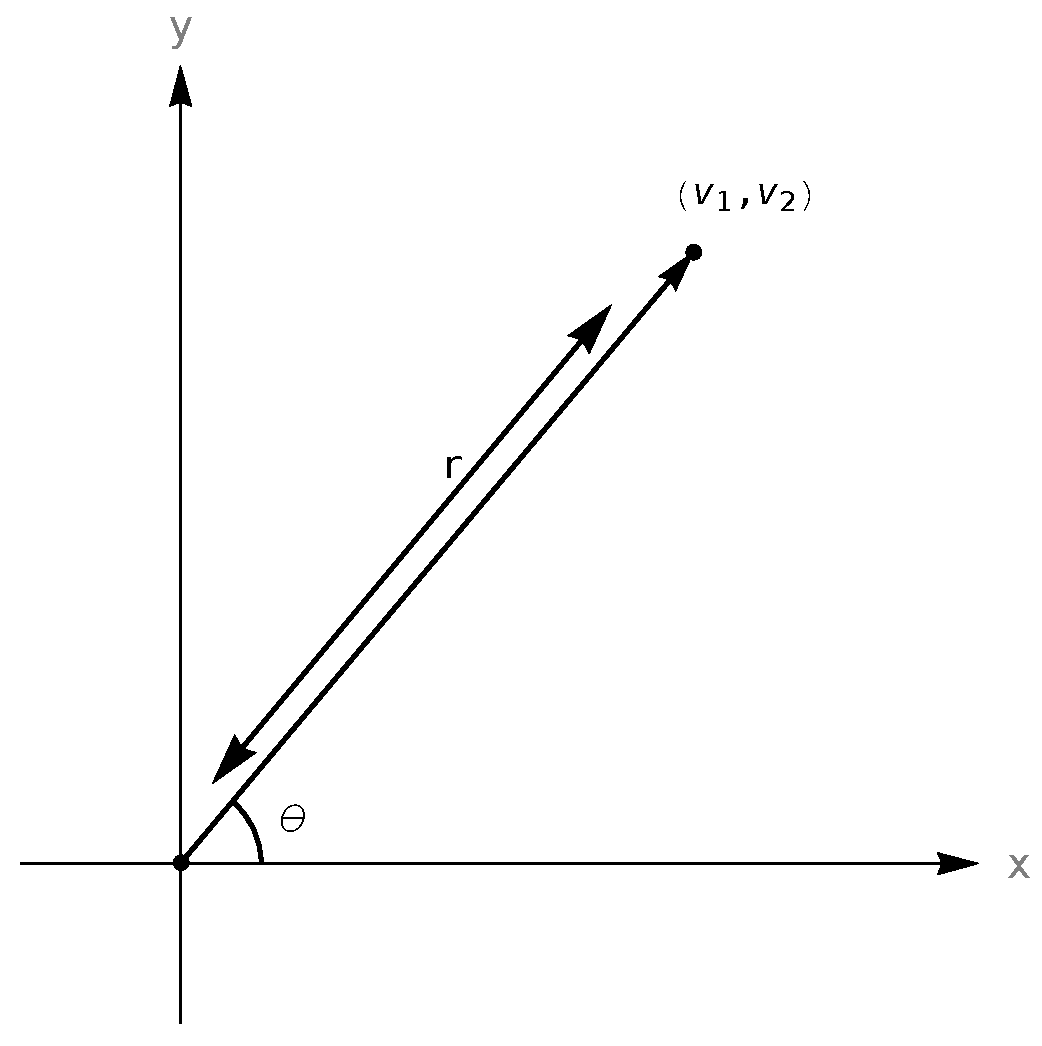
\includegraphics[width=0.35\textwidth]{fig_vector_8}
	\caption{The $\vec{v}= \left(v_1,v_2\right)$ in standard position. }
	\label{fig_vector_8}
	\end{center}
\end{figure}

\ifvc
Plotting a vector in standard position enables us to more easily quantify the concepts of magnitude and direction of the vector. The magnitude of $\vec{v}$, which we said earlier was the length of the directed line segment, is $r = \sqrt{v_1^2 + v_2^2}$ and is denoted by $\| \vec{v} \|$. It holds that $v_1 = r \cos(\theta) = \| \vec{v} \| \cos(\theta)$ and $v_2  = r \sin(\theta) = \| \vec{v} \| \sin(\theta)$. From the definition of scalar multiplication and vector equality, we get

\[ \begin{array}{rcl} \vec{v} & = & \left( v_1 , v_2  \right) \\ [3pt]
& = & \left( \| \vec{v} \| \cos(\theta), \| \vec{v} \| \sin(\theta) \right) \\ [3pt]
& = &  \| \vec{v} \| \left( \cos(\theta),\sin(\theta) \right). \\ \end{array} \]
This motivates the following definition.

\index{magnitude}\index[aut]{grootte}\index{direction}\index[aut]{richting}
\begin{definition}[Magnitude and direction of a vector] \label{polarformvector} 
	Suppose $\vec{v}$ is a vector with component form $\vec{v} =\left( v_1 , v_2  \right)$. 
	\begin{itemize}
		
		\item  The \textbf{magnitude} (\textit{grootte}) \index{magnitude} \index[aut]{grootte} of $\vec{v}$, denoted $\| \vec{v} \|$, is given by 
		$$\| \vec{v} \| = r =   \sqrt{v_1^2 + v_2^2}\,.$$
		
		\item If $\vec{v} \neq \vec{0}$,  the \textbf{(vector) direction} (\textit{richting}) \index{direction} \index[aut]{richting} of $\vec{v}$, denoted $\hat{v}$ is given by  
		$$\hat{v} = \left( \cos(\theta), \sin(\theta) \right)\,.$$
		
	\end{itemize}
	
\end{definition}

\fi

\ifcourse
Plotting a vector in standard position enables us to more easily quantify the concepts of magnitude and direction of the vector. We can convert the point $\left(v_1,v_2\right)$ in rectangular coordinates to a pair $(r,\theta)$ in polar coordinates where $r \geq 0$.  The magnitude of $\vec{v}$, which we said earlier was the length of the directed line segment, is $r = \sqrt{v_1^2 + v_2^2}$ and is denoted by $\| \vec{v} \|$.  From Theorem~\ref{cosinesinecircle}, we know $v_1 = r \cos(\theta) = \| \vec{v} \| \cos(\theta)$ and $v_2  = r \sin(\theta) = \| \vec{v} \| \sin(\theta)$. From the definition of scalar multiplication and vector equality, we get

\[ \begin{array}{rcl} \vec{v} & = & \left( v_1 , v_2  \right) \\ [3pt]
															& = & \left( \| \vec{v} \| \cos(\theta), \| \vec{v} \| \sin(\theta) \right) \\ [3pt]
													    & = &  \| \vec{v} \| \left( \cos(\theta),\sin(\theta) \right). \\ \end{array} \]
This motivates the following definition.

\index{magnitude}\index[aut]{grootte}\index{direction}\index[aut]{richting}
\begin{definition}[Magnitude and direction of a vector] \label{polarformvector} 
 Suppose $\vec{v}$ is a vector with component form $\vec{v} =\left( v_1 , v_2  \right)$.  Let $(r,\theta)$ be a polar representation of the point with rectangular coordinates $\left(v_1 ,v_2  \right)$ with $r \geq 0$.
\begin{itemize}

\item  The \textbf{magnitude} (\textit{grootte}) \index{magnitude} \index[aut]{grootte} of $\vec{v}$, denoted $\| \vec{v} \|$, is given by 
$$\| \vec{v} \| = r =   \sqrt{v_1^2 + v_2^2}\,.$$

\item If $\vec{v} \neq \vec{0}$,  the \textbf{(vector) direction} (\textit{richting}) \index{direction} \index[aut]{richting} of $\vec{v}$, denoted $\hat{v}$ is given by  
$$\hat{v} = \left( \cos(\theta), \sin(\theta) \right)\,.$$

\end{itemize}

\end{definition}

\fi

Both magnitude and direction of a vector come along with a few important properties.


\begin{itemize}

\item It holds  that $\| \vec{v} \| \geq 0$ and $\| \vec{v} \| = 0$ if and only if $\vec{v} = \vec{0}$.

\item  For all scalars $k$, it holds that 
$$
\| k \, \vec{v} \| = |k| \, \| \vec{v} \|\,.
$$

\item  If $\vec{v} \neq \vec{0}$ then $\vec{v} = \| \vec{v} \|\, \hat{v}$, so that 
\begin{equation}
\hat{v} = \left(\frac{1}{\|\vec{v}\|}\right) \vec{v}\,.
\label{propdir3}
\end{equation}
\end{itemize}

% \ifcourse
% \ifanalysis
% 
% The proof of the first property is a direct consequence of the definition of $\| \vec{v} \|$.  If $\vec{v}  = \left( v_1 ,v_2\right)$, then $\| \vec{v} \| = \sqrt{v_1^2 + v_2^2},$ which is by definition greater than or equal to $0$.  Moreover, $\sqrt{v_1^2 + v_2^2} = 0$ if and only of $v_1^2 + v_2^2 = 0$ if and only if $v_1 = v_2 = 0$.  Hence, $\| \vec{v} \| = 0$ if and only if $\vec{v} = \left(0,0\right) =  \vec{0}$, as required.

% \smallskip

% The second property is a result of the definition of magnitude and scalar multiplication along with a property of radicals. If $\vec{v} = \left( v_1 ,v_2\right)$ and $k$ is a scalar then 

% \[ \begin{array}{rcll}

% \| k \, \vec{v} \| & = & \| k \left( v_1, v_2\right) \| & \\ [3pt]
% 									 & = & \| \left(kv_1,kv_2\right)\| & \quad\text{(Definition of scalar multiplication.)} \\ [3pt]
% 									 & = & \sqrt{\left(kv_1\right)^2 + \left(kv_2\right)^2} & \quad\text{(Definition of magnitude.)} \\ [3pt]
% 									 & = & \sqrt{k^2v_1^2 + k^2v_2^2} & \\[3pt]
% 									 & = & \sqrt{k^2(v_1^2+v_2^2)} & \\ [3pt]
% 									 & = & \sqrt{k^2} \sqrt{v_1^2+v_2^2} & \quad\text{(Product rule for radicals.)} \\ [3pt]
% 									 & = & |k| \sqrt{v_1^2+v_2^2} & \quad\text{(Since $\sqrt{k^2} = |k|$.)} \\
% 									 & = & |k| \| \vec{v} \| & \\
% \end{array} \]

% \smallskip

% Finally, the equation $\vec{v} = \| \vec{v} \| \hat{v}$  is a consequence of the definitions of $\| \vec{v} \|$ and $\hat{v}$.  This equation says that any given vector is the product of its magnitude and its direction. Equation~\eqref{propdir3} is a result of solving $\vec{v} = \| \vec{v} \| \hat{v}$  for $\hat{v}$ by multiplying both sides of the equation by $\| \vec{v} \|^{-1}$ and using the properties of scalar multiplication of vectors.


% 
% \fi
% \fi

\begin{example} \label{polarformvecex} 
\ifcourse
\begin{enumerate}
\item  Find the polar representation of the vector $\vec{v} = \left(3, -3\sqrt{3}\right)$, assuming that $0 \leq \theta < 2\pi$.

\item For the vectors $\vec{v} = \left(3,4\right)$ and $\vec{w} = \left(1, -2\right)$, find the following.

\begin{multicols}{4}

\begin{enumerate}

\item  $\hat{v}$

\item  $\| \vec{v} \| -2 \|\vec{w}\|$

\item  $\| \vec{v} -2\vec{w}\|$

\item  $\| \hat{w} \|$ \label{preludetounitvector}

\end{enumerate}

\end{multicols}
\end{enumerate}
\fi

\ifvc
For the vectors $\vec{v} = \left(3,4\right)$ and $\vec{w} = \left(1, -2\right)$, find the following.
	\begin{multicols}{4}	
		\begin{enumerate}
			
			\item  $\hat{v}$
			
			\item  $\| \vec{v} \| -2 \|\vec{w}\|$
			
			\item  $\| \vec{v} -2\vec{w}\|$
			
			\item  $\| \hat{w} \|$ \label{preludetounitvector}
			
		\end{enumerate}	
	\end{multicols}

\fi

\pagebreak
\xhrulefill{gray}{2.5pt}Solution \xhrulefill{gray}{2.5pt}

\ifcourse
\begin{enumerate}

\item  For $\vec{v} =  \left(3, -3\sqrt{3}\right)$, we get $\| \vec{v} \| = \sqrt{(3)^2+(-3\sqrt{3})^2} = 6$.  We can find the $\theta$ we are after by converting the point with rectangular coordinates $(3, -3\sqrt{3})$ to polar form $(r,\theta)$ where $r = \|\vec{v}\| >0$.  This leads to $\tan(\theta) = -3\sqrt{3}/3 = -\sqrt{3}$. Since  $(3, -3\sqrt{3})$ is a point in Quadrant IV, $\theta$ is a Quadrant IV angle.  Hence, we pick $\theta = \frac{5\pi}{3}$.  

\item  \begin{enumerate} \item  Since we are given the component form of $\vec{v}$, we will use Equation~\eqref{propdir3}.  For $\vec{v} = \left(3,4\right)$, we have $\| \vec{v} \| = \sqrt{3^2+4^2} = \sqrt{25} = 5$.  Hence, $\hat{v} = \frac{1}{5} \left( 3, 4 \right) = \left(\frac{3}{5}, \frac{4}{5}\right)$.


\item  We already know that $\| \vec{v} \| = 5$, so to find  $\| \vec{v} \| -2 \|\vec{w}\|$, we need only find $\| \vec{w} \|$.  Since $\vec{w} = \left(1, -2\right)$, we get $\| \vec{w} \| = \sqrt{1^2+(-2)^2} = \sqrt{5}$.  Hence, $\| \vec{v} \| -2 \|\vec{w}\| = 5 - 2\sqrt{5}$.

\item  Our first step is to find the component form of the vector $\vec{v} - 2\vec{w}$.  As such, we get $\vec{v} - 2 \vec{w} = \left(3,4\right) - 2\left(1,-2\right) = \left(1, 8\right)$.  Hence,  $\| \vec{v} -2\vec{w}\| =  \| \left(1, 8\right)\| = \sqrt{1^2+8^2} = \sqrt{65}$.


\item  To find $\| \hat{w} \|$, we first need $\hat{w}$.  Using Equation~\eqref{propdir3} along with $\| \vec{w} \| = \sqrt{5}$,  we get  
$$\hat{w} = \frac{1}{\sqrt{5}} \left(1, -2\right) = \left( \frac{1}{\sqrt{5}}, -\frac{2}{\sqrt{5}}\right)  = \left( \frac{\sqrt{5}}{5}, -\frac{2\sqrt{5}}{5}\right)\,.$$
 Hence, 
$$\| \hat{w} \| = \sqrt{\left( \frac{\sqrt{5}}{5}\right)^2 + \left(-\frac{2\sqrt{5}}{5}\right)^2} = \sqrt{\frac{5}{25} + \frac{20}{25}} = \sqrt{1} = 1\,.$$ 


\end{enumerate}

\end{enumerate}
\fi

\ifvc
\begin{enumerate} \item  Since we are given the component form of $\vec{v}$, we will use Equation~\eqref{propdir3}.  For $\vec{v} = \left(3,4\right)$, we have $\| \vec{v} \| = \sqrt{3^2+4^2} = \sqrt{25} = 5$.  Hence, $\hat{v} = \frac{1}{5} \left( 3, 4 \right) = \left(\frac{3}{5}, \frac{4}{5}\right)$.
	
	
	\item  We already know that $\| \vec{v} \| = 5$, so to find  $\| \vec{v} \| -2 \|\vec{w}\|$, we need only find $\| \vec{w} \|$.  Since $\vec{w} = \left(1, -2\right)$, we get $\| \vec{w} \| = \sqrt{1^2+(-2)^2} = \sqrt{5}$.  Hence, $\| \vec{v} \| -2 \|\vec{w}\| = 5 - 2\sqrt{5}$.
	
	\item  Our first step is to find the component form of the vector $\vec{v} - 2\vec{w}$.  As such, we get $\vec{v} - 2 \vec{w} = \left(3,4\right) - 2\left(1,-2\right) = \left(1, 8\right)$.  Hence,  $\| \vec{v} -2\vec{w}\| =  \| \left(1, 8\right)\| = \sqrt{1^2+8^2} = \sqrt{65}$.
	
	
	\item  To find $\| \hat{w} \|$, we first need $\hat{w}$.  Using Equation~\eqref{propdir3} along with $\| \vec{w} \| = \sqrt{5}$,  we get  
	$$\hat{w} = \frac{1}{\sqrt{5}} \left(1, -2\right) = \left( \frac{1}{\sqrt{5}}, -\frac{2}{\sqrt{5}}\right)  = \left( \frac{\sqrt{5}}{5}, -\frac{2\sqrt{5}}{5}\right)\,.$$
	Hence, 
	$$\| \hat{w} \| = \sqrt{\left( \frac{\sqrt{5}}{5}\right)^2 + \left(-\frac{2\sqrt{5}}{5}\right)^2} = \sqrt{\frac{5}{25} + \frac{20}{25}} = \sqrt{1} = 1\,.$$ 
	
	
\end{enumerate}
\fi

\end{example}

The process exemplified in Example \ref{polarformvecex} by which we take information about the magnitude and direction of a vector and find the component form of a vector is called \textbf{resolving} a vector into its components. 


\section{Unit vectors}
\label{sec_eenheidsvect}
 Vectors with length 1 are called unit vectors and are very important in algebra. 



\begin{definition}[Unit vector] \label{unitvectordefn} \index{vector ! unit vector} \index{unit vector} \index[aut]{vector ! eenheidsvector} \index[aut]{eenheidsvector} 
Let $\vec{v}$ be a vector. If $\| \vec{v} \| = 1$, we say that $\vec{v}$ is a \textbf{unit vector} (\textit{eenheidsvector}).

\end{definition}

If $\vec{v}$ is a unit vector, then necessarily,  
$$
\vec{v} = \| \vec{v} \| \hat{v} = 1 \cdot \hat{v} = \hat{v}.
$$
 Conversely, it can be shown that 
$$\hat{v} = \left( \frac{1}{\| \vec{v} \|} \right) \vec{v}$$
 is a unit vector for any nonzero vector $\vec{v}$.   The process of multiplying a nonzero vector by the factor $\| \vec{v} \|^{-1}$ to produce a unit vector is called \index{vector ! normalization} \index[aut]{vector ! normeren}\textbf{normalizing} (\textit{normeren}) the vector and the resulting vector $\hat{v}$ is called the `unit vector in the direction of $\vec{v}$'.  The terminal points of unit vectors, when plotted in standard position, lie on the unit circle.  As a result, we may visualize normalizing a nonzero vector $\vec{v}$ as shrinking its terminal point, when plotted in standard position, back to the unit circle.  In practice, if $\vec{v}$ is a unit vector we write it as $\hat{v}$ (Figure~\ref{fig_vector_9}). 

\begin{figure}[H]
	\begin{center}
			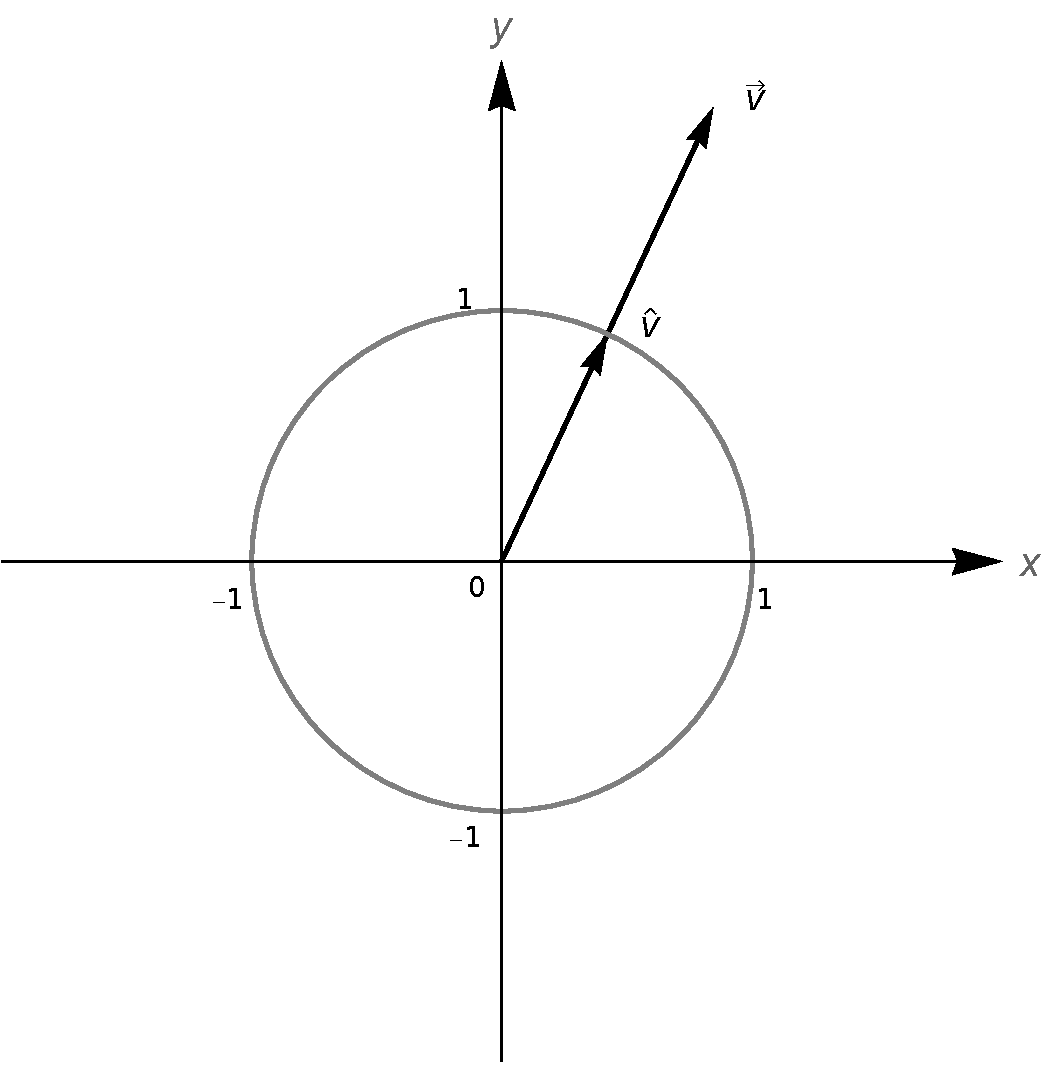
\includegraphics[width=0.35\textwidth]{fig_vector_9}
	\caption{Vector normalisation $\hat{v} = \left( \frac{1}{\| \vec{v} \|} \right) \vec{v}$. }
	\label{fig_vector_9}
	\end{center}
\end{figure}


Of all of the unit vectors, the so-called  \index{vector ! principal unit vectors}\index[aut]{basisvector}\textbf{principal unit vectors} (\textit{basis eenheidsvector}) deserve special attention. In two dimensions, they are given by

\begin{itemize}

\item The vector $\hat{\imath} = \left(1,0\right),$

\item The vector $\hat{\jmath} = \left(0,1\right).$

\end{itemize}


We may think of the vector $\hat{\imath}$ as representing the positive $x$-direction, while $\hat{\jmath}$ represents the positive $y$-direction.  Consequently, the coordinate axes $x$ and $y$ are the axes in the direction of $\hat{\imath}$ and $\hat{\jmath}$, respectively. Together, $\hat{\imath}$ and $\hat{\jmath}$ make up the so-called \index{standard basis}\index[aut]{standaardbasis}\textbf{standard basis} (\textit{standaardbasis}) for the Euclidean plane. Having introduced principal unit vectors, we are now ready to get up to the following decomposition theorem.


\begin{theorem}[Principal vector decomposition theorem] \label{ijdecomp}  

 Let $\vec{v}$ be a vector with component form  $\vec{v} = \left( v_1 ,v_2\right)$. Then $\vec{v} = v_1 \hat{\imath} + v_2 \hat{\jmath}$. \index{vector ! decomposition theorem}


\end{theorem}

\ifcourse
\ifanalysis

\begin{proof}
The proof of this theorem is straightforward. Since $\hat{\imath} = \left(1,0\right)$ and $\hat{\jmath} = \left( 0,1\right)$, we have from the definition of scalar multiplication and vector addition that  

\[v_1 \hat{\imath} + v_2 \hat{\jmath} = v_1\left(1,0\right) + v_2\left(0,1\right) = \left(v_1,0\right) + \left(0,v_2\right) = \left(v_1,v_2\right) = \vec{v}\]

Geometrically, the situation looks like the diagram in Figure~\ref{fig_vector_10}.
\end{proof}

\begin{figure}
	\begin{center}
			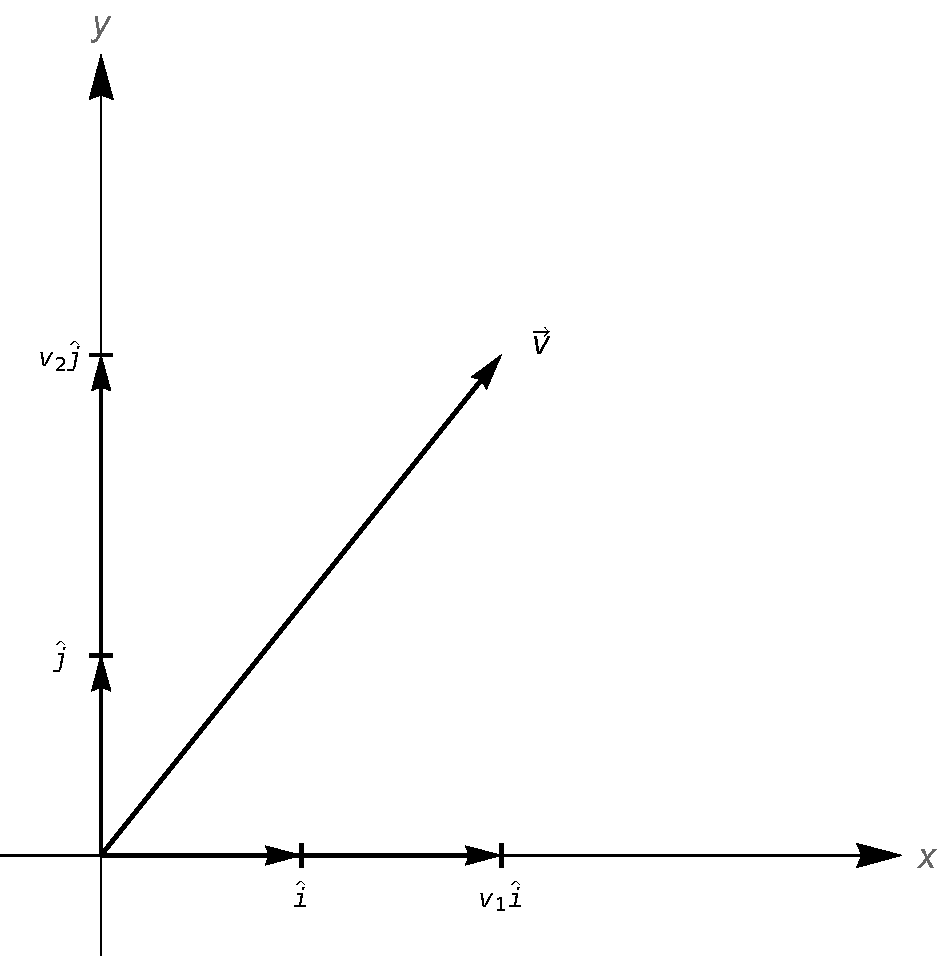
\includegraphics[width=0.4\textwidth]{fig_vector_10}
	\caption{$\vec{v} = \left(v_1,v_2\right) = v_1\hat{\imath} + v_2 \hat{\jmath}$. }
	\label{fig_vector_10}
	\end{center}
\end{figure}


We conclude this section with a classic example that demonstrates how vectors are used to model forces.  A force is defined as a push or a pull.   The intensity of the push or pull is the magnitude of the force, and is  measured in Newton (N).

\begin{example} \label{forceex}
  A  speaker exerting a fore by gravity of 50 Newton is  suspended from the ceiling by two support braces.   If one of them makes a $60^{\circ}$ angle with the ceiling and the other makes a $30^{\circ}$ angle with the ceiling, what are the tensions on each of the supports?


\xhrulefill{gray}{2.5pt}Solution \xhrulefill{gray}{2.5pt}

The problem is sketched schematically in Figure~\ref{fig_vector_11a} and  the corresponding vector diagram is given in Figure~\ref{fig_vector_11b}. 

\begin{figure}[H]
\centering
%\right)isebox{0.5cm}{
\centerline{
\subfigure[\label{fig_vector_11a}]{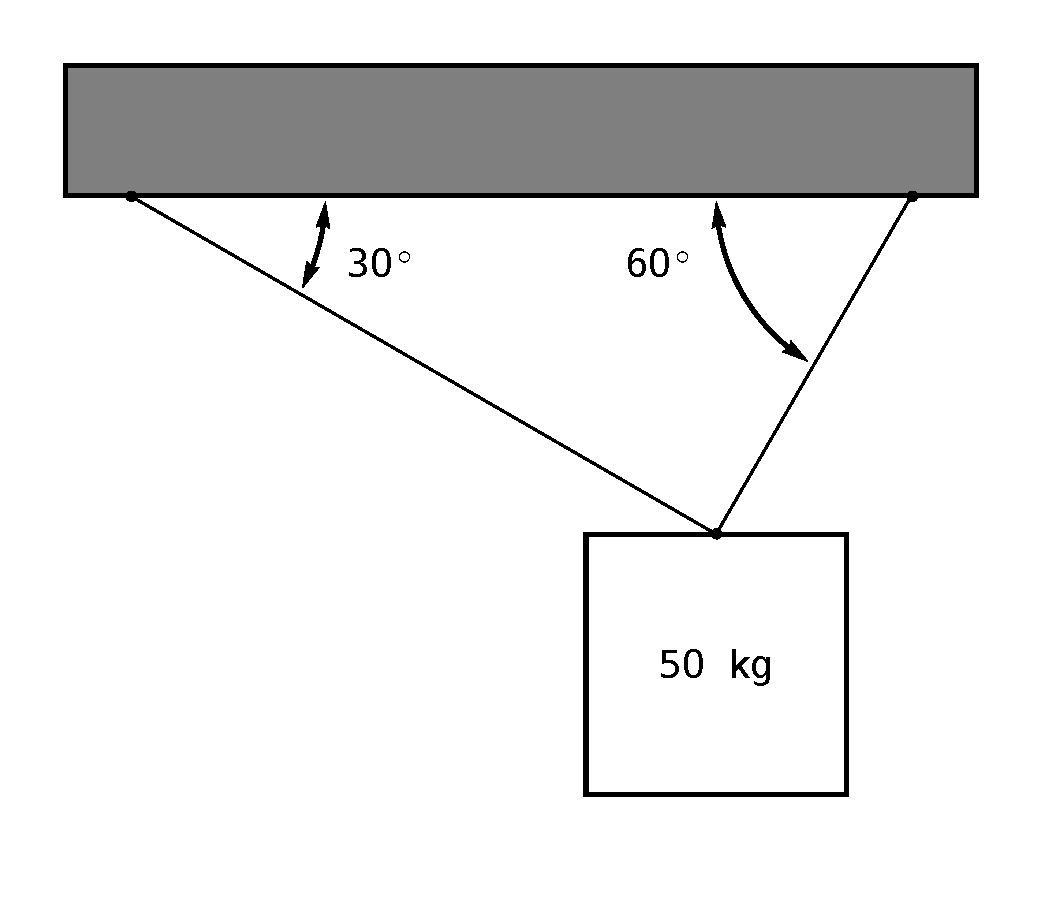
\includegraphics[width=0.43\textwidth]{fig_vector_11a}}
\hspace{0.1cm}
\subfigure[\label{fig_vector_11b}]{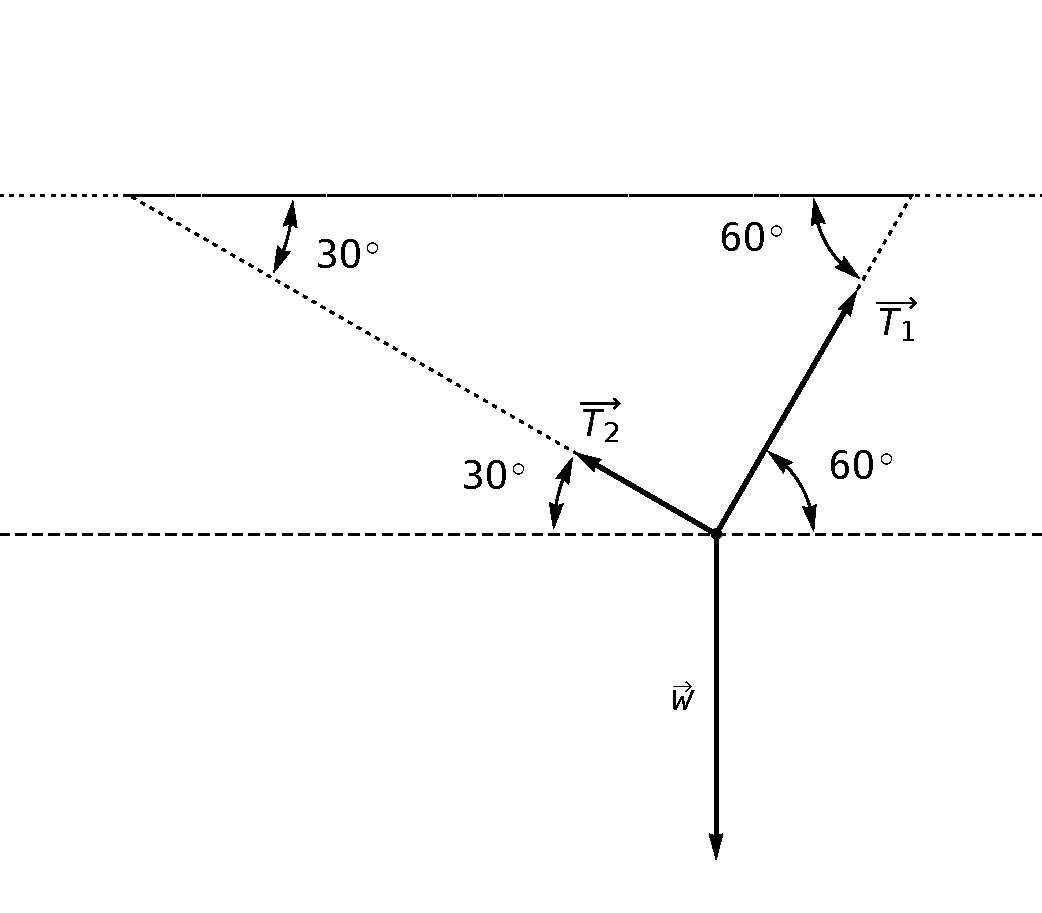
\includegraphics[width=0.43\textwidth]{fig_vector_11b}}
}
\caption{Schematic representation and corresponding vector diagram for the problem in Example~\ref{forceex}. }

\end{figure}

We have three forces acting on the speaker:  the weight of the speaker, which we will call  $\vec{w}$, pulling the speaker directly downward, and the forces on the support rods, which we will call $\overrightarrow{\mathbf{T_1}}$ and $\overrightarrow{\mathbf{T_2}}$ (for tensions) acting upward at angles $60^{\circ}$ and $30^{\circ}$, respectively.  We are looking for the tensions on the support, which are the magnitudes  $\| \overrightarrow{\mathbf{T_1}} \|$  and  $\| \overrightarrow{\mathbf{T_2}}\|$.   In order for the speaker to remain stationary, we require  $\vec{w} + \overrightarrow{\mathbf{T_1}} + \overrightarrow{\mathbf{T_2}} = \vec{0}$.  Viewing the common initial point of these vectors as the origin and the dashed line as the $x$-axis, we get the component representations for the three vectors involved. We can model the weight of the speaker as a vector pointing directly downwards with a magnitude of $50$ Newton.  That is,  $\| \vec{w} \| = 50$ and $\hat{w} = -\hat{\jmath} = \left(0,-1\right)$.  Hence, $\vec{w} = 50\left(0,-1\right) = \left(0,-50\right)$.  For the force in the first support, we get
 
\[ \begin{array}{rcl}

\overrightarrow{\mathbf{T_1}} &  = &  \| \overrightarrow{\mathbf{T_1}} \|\left(\cos\left(60^{\circ}\right), \sin\left(60^{\circ}\right)\right) \\ [8pt]
                            & =  & \left( \dfrac{\| \overrightarrow{\mathbf{T_1}} \|}{2} , \dfrac{\| \overrightarrow{\mathbf{T_1}} \|\sqrt{3}}{2}\right). \\ \end{array} \]
                            
For the second support, we note that the angle $30^{\circ}$ is measured from the negative $x$-axis, so the angle needed to write $\overrightarrow{\mathbf{T_2}}$ in component form is $150^{\circ}$.  Hence

\[ \begin{array}{rcl}

\overrightarrow{\mathbf{T_2}} & = & \| \overrightarrow{\mathbf{T_2}} \|\left(\cos\left(150^{\circ}\right), \sin\left(150^{\circ}\right)\right)\\ [8pt]
                           & =  & \left(-\dfrac{\| \overrightarrow{\mathbf{T_2}} \|\sqrt{3}}{2}, \dfrac{\| \overrightarrow{\mathbf{T_2}} \|}{2} \right). \\ \end{array} \]
                           
The requirement $\vec{w} + \overrightarrow{\mathbf{T_1}} + \overrightarrow{\mathbf{T_2}} = \vec{0}$ gives us the following  vector equation.
 
 \[ \begin{array}{rcl}
 
\vec{w} + \overrightarrow{\mathbf{T_1}} + \overrightarrow{\mathbf{T_2}} &  = &  \vec{0}  \\ [8pt]

\left(0,-50\right) + \left( \dfrac{\| \overrightarrow{\mathbf{T_1}}  \|}{2} , \dfrac{\| \overrightarrow{\mathbf{T_1}}  \|\sqrt{3}}{2}\right) +  \left(-\dfrac{\| \overrightarrow{\mathbf{T_2}} \|\sqrt{3}}{2}, \dfrac{\| \overrightarrow{\mathbf{T_2}} \|}{2} \right) & = & \left(0, 0\right) \\ [8pt]

\left( \dfrac{\| \overrightarrow{\mathbf{T_1}}  \|}{2} -\dfrac{\| \overrightarrow{\mathbf{T_2}} \|\sqrt{3}}{2}, \dfrac{\| \overrightarrow{\mathbf{T_1}}  \|\sqrt{3}}{2} +  \dfrac{\| \overrightarrow{\mathbf{T_2}} \|}{2} -50  \right) & = & \left(0, 0\right)  \\ 
\end{array} \]

Equating the corresponding components of the vectors on each side,  we get a system of linear equations in the variables $\| \overrightarrow{\mathbf{T_1}} \| $ and   $\| \overrightarrow{\mathbf{T_2}} \|$.


\begin{eqnarray}
  \dfrac{\| \overrightarrow{\mathbf{T_1}}  \|}{2} -\dfrac{\| \overrightarrow{\mathbf{T_2}} \|\sqrt{3}}{2} & = & 0 \label{forceexeq1}\\ [8pt]  
	 \dfrac{\| \overrightarrow{\mathbf{T_1}}  \|\sqrt{3}}{2} +  \dfrac{\| \overrightarrow{\mathbf{T_2}}  \|}{2} -50 & = & 0 \label{forceexeq2}
	\end{eqnarray}

From Equation~\eqref{forceexeq1}, we get $\| \overrightarrow{\mathbf{T_1}}  \| = \| \overrightarrow{\mathbf{T_2}} \| \sqrt{3}$.  Substituting that into Equation~\eqref{forceexeq2} gives 
$$\frac{(\| \overrightarrow{\mathbf{T_2}}  \| \sqrt{3})\sqrt{3}}{2} +  \frac{\| \overrightarrow{\mathbf{T_2}}  \|}{2} - 50 = 0$$
which yields $2\| \overrightarrow{\mathbf{T_2}} \| - 50 =0.$
Hence, $\| \overrightarrow{\mathbf{T_2}} \| = 25$ Newton and  $\| \overrightarrow{\mathbf{T_1}} \| = \| \overrightarrow{\mathbf{T_2}}  \| \sqrt{3} = 25 \sqrt{3}$ Newton.

\end{example}


\fi
\fi


\section{The dot product}
\label{sec_scalair_product}
In Section~\ref{sec_vector_arith}, we learned how add and subtract vectors and how to multiply vectors by scalars.  Here, we will see how to multiply vectors.  We begin with the following definition.


\begin{definition}[Dot product] \label{dotproductdefn}    
Suppose $\vec{v}$ and $\vec{w}$ are vectors whose component forms are $\vec{v} = \left(v_1,v_2\right)$ and $\vec{w} = \left(w_1,w_2\right)$.  The \textbf{dot product}\ (\textit{scalair product})\index{vector ! dot product}\index{vector ! scalar product}\index{dot product}\index[aut]{scalair product}\index[aut]{inproduct} \index[aut]{vector ! scalair product}\index[aut]{vector ! inproduct} of $\vec{v}$ and $\vec{w}$ is given by

\[ \vec{v} \cdot \vec{w} = \left(v_1,v_2\right) \cdot \left(w_1,w_2\right) = v_1w_1 + v_2w_2. \].

\end{definition}


For example, let $\vec{v} = \left(3,4\right)$ and $\vec{w} = \left(1,-2\right)$.  Then $\vec{v} \cdot \vec{w} = \left(3,4\right) \cdot \left(1,-2\right) =  (3)(1) + (4)(-2) = -5$. Note that the dot product takes two vectors and produces a scalar. The dot product enjoys the following properties for all vectors $\vec{u}$, $\vec{v}$ and $\vec{w}$ and scalar $k$.

\begin{itemize}

\item  \textbf{Commutative property:}  
 $$\vec{v} \cdot \vec{w} = \vec{w} \cdot \vec{v}\,,$$

\item  \textbf{Distributive property:}  
 $$\vec{u} \cdot \left(\vec{v} + \vec{w}\right) = \vec{u} \cdot \vec{v} + \vec{u} \cdot \vec{w}\,,$$

\item  \textbf{Scalar property:}  
 $$ (k \vec{v}) \cdot \vec{w} = k(\vec{v} \cdot \vec{w}) = \vec{v} \cdot (k \vec{w})\,,$$

\item  \textbf{Relation to magnitude:}  
 $$\vec{v} \cdot \vec{v} = \| \vec{v} \|^2\,.$$ 

\end{itemize}
\index{distributivity}\index[aut]{distributiviteit}\index{associativity}\index[aut]{associativiteit}


\ifcourse
Like most of the theorems involving vectors, the proof of these properties amounts to using the definition of the dot product and properties of real number arithmetic.  
\ifanalysis

\begin{proof}
To show the commutative property for instance, let $\vec{v} = \left(v_1,v_2\right)$ and $\vec{w} = \left(w_1,w_2\right)$.  Then

\[ \begin{array}{rcll}

\vec{v} \cdot \vec{w} & = & \left(v_1,v_2\right)  \cdot \left(w_1,w_2\right)  & \\ [3pt]
										 & = & v_1w_1 + v_2w_2 & \quad\text{(Definition of dot product.)} \\ [3pt]
										 & = & w_1v_1 + w_2v_2 & \quad\text{(Commutativity of real number multiplication.)} \\ [3pt]
										 & = & \left(w_1,w_2\right)  \cdot  \left(v_1,v_2\right)  & \quad\text{(Definition of dot product.)} \\ [3pt]
										 & = & \vec{w} \cdot \vec{v} & \\ \end{array} \]

The distributive property is proved similarly.

\smallskip

For the scalar property, assume that $\vec{v} = \left(v_1,v_2\right)$ and $\vec{w} = \left(w_1,w_2\right)$ and $k$ is a scalar.  Then

\[ \begin{array}{rcll}

(k\vec{v}) \cdot \vec{w} & = & \left(k \left(v_1,v_2\right) \right) \cdot \left(w_1,w_2\right) & \\ [3pt]
												 & = &  \left(kv_1,kv_2\right)  \cdot \left(w_1,w_2\right) & \quad\text{(Definition of scalar multiplication.)} \\ [3pt]
												 & = & (kv_1)(w_1) + (kv_2)(w_2) & \quad\text{(Definition of dot product.)} \\ [3pt]
												 & = & k(v_1w_1) + k(v_2w_2) & \quad\text{(Associativity of real number multiplication.)} \\ [3pt]
												 & = & k(v_1w_1 + v_2w_2) & \quad\text{(Distributive law of real numbers.)} \\ [3pt]
												 & = & k \left(v_1,v_2\right)  \cdot \left(w_1,w_2\right) & \quad\text{(Definition of dot product.)} \\ [3pt]
												 & = & k (\vec{v} \cdot \vec{w}) & \\ \end{array} \]
\enlargethispage{.25in} The property $k(\vec{v} \cdot \vec{w}) = \vec{v} \cdot (k \vec{w})$ can be proved similarly

For the last property, we note that if  $\vec{v} = \left(v_1,v_2\right)$, then $\vec{v} \cdot \vec{v} = \left(v_1,v_2\right) \cdot \left(v_1,v_2\right) = v_1^2 + v_2^2 = \|\vec{v}\|^2$ (Definition~\ref{polarformvector}).
\end{proof}

\fi
\fi

% \ifcourse
% \ifanalysis
% The following example puts these properties to good use. 

% \begin{example}  \label{dotprodpropex} 
%  Prove the identity:  $\| \vec{v} - \vec{w} \|^2 =  \|\vec{v}\|^2  -2 (\vec{v}\cdot\vec{w}) + \|\vec{w}\|^2$.

% \xhrulefill{gray}{2.5pt}Solution \xhrulefill{gray}{2.5pt}

%  We begin by rewriting  $\| \vec{v} - \vec{w} \|^2$ in terms of the dot product.

% \[ \begin{array}{rcl}

% \| \vec{v} - \vec{w} \|^2 & = & (\vec{v} - \vec{w}) \cdot (\vec{v} - \vec{w})  \\ [3pt]
% % 													& = & (\vec{v} + [-\vec{w}]) \cdot (\vec{v} + [-\vec{w}]) \\ [3pt]										
% 													& = & \vec{v} \cdot (\vec{v} + [-\vec{w}])  + [-\vec{w}] \cdot (\vec{v} + [-\vec{w}]) \\ [3pt]
% 													& = & \vec{v} \cdot \vec{v} + \vec{v} \cdot [-\vec{w}] + [-\vec{w}]\cdot \vec{v} + [-\vec{w}]\cdot[-\vec{w}] \\ [3pt]
% 													& = & \vec{v} \cdot \vec{v} + \vec{v} \cdot [(-1)\vec{w}] + [(-1)\vec{w}]\cdot \vec{v} + [(-1)\vec{w}]\cdot[(-1)\vec{w}] \\ [3pt]	
% 													& = & \vec{v} \cdot \vec{v} + (-1)(\vec{v} \cdot \vec{w}) + (-1)(\vec{w} \cdot \vec{v}) + [(-1)(-1)](\vec{w}\cdot\vec{w}) \\ [3pt]	
% 													& = & \vec{v} \cdot \vec{v} + (-1)(\vec{v} \cdot \vec{w}) + (-1)(\vec{v} \cdot \vec{w}) + \vec{w}\cdot\vec{w} \\ [3pt]
% 												  & = & \vec{v} \cdot \vec{v} -2(\vec{v} \cdot \vec{w}) + \vec{w}\cdot\vec{w} \\ [3pt]
% 													& = & \|\vec{v}\|^2-2(\vec{v} \cdot \vec{w}) +\|\vec{w}\|^2
													
% \end{array}\]
%Hence,  $\| \vec{v} - \vec{w} \|^2 =  \|\vec{v}\|^2  -2 (\vec{v}\cdot\vec{w}) + \|\vec{w}\|^2$ as required.  

% \end{example} 


% The identity verified in this example plays a large role in the development of the geometric properties of the dot product, which we now explore. 
% \fi
% \fi

 We now explore the geometric properties of the dot product. Suppose for that purpose  $\vec{v}$ and $\vec{w}$ are two nonzero vectors. If we draw $\vec{v}$ and $\vec{w}$ with the same initial point, we define the angle between $\vec{v}$ and $\vec{w}$ to be the angle $\theta$ determined by the rays containing the vectors $\vec{v}$ and $\vec{w}$, as illustrated in Figure~\ref{fig_vector_12}.  We require $0 \leq \theta \leq \pi$. 

\begin{figure}[H]
\centering
%\right)isebox{0.5cm}{
\centerline{
\subfigure[$\theta=0$\label{fig_vector_12a}]{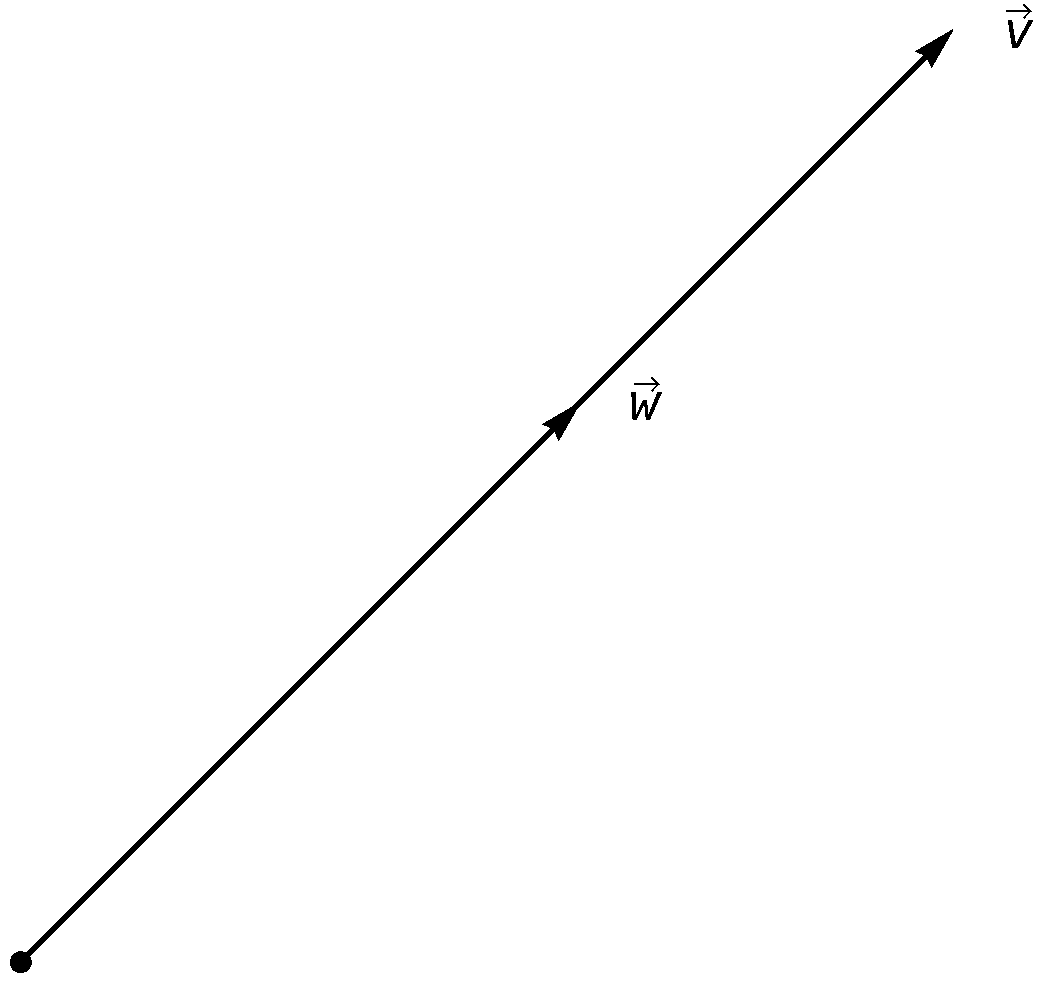
\includegraphics[width=0.3\textwidth]{fig_vector_12a}}
\hspace{0.1cm}
\subfigure[$0<\theta<\pi$\label{fig_vector_12b}]{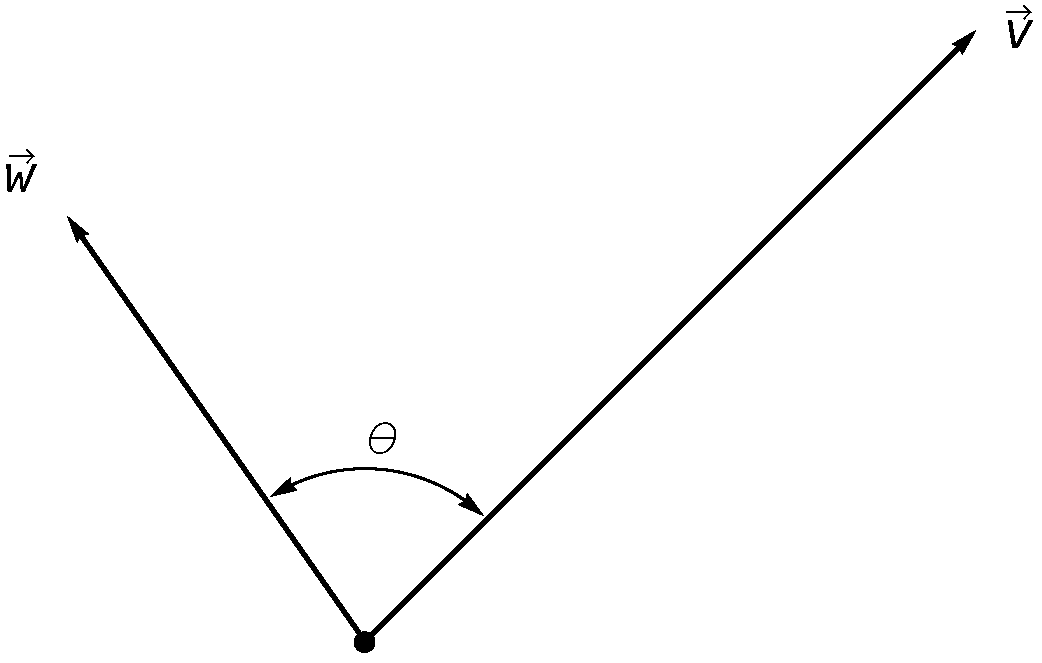
\includegraphics[width=0.3\textwidth]{fig_vector_12b}}
\hspace{0.1cm}
\subfigure[$\theta=\pi$\label{fig_vector_12c}]{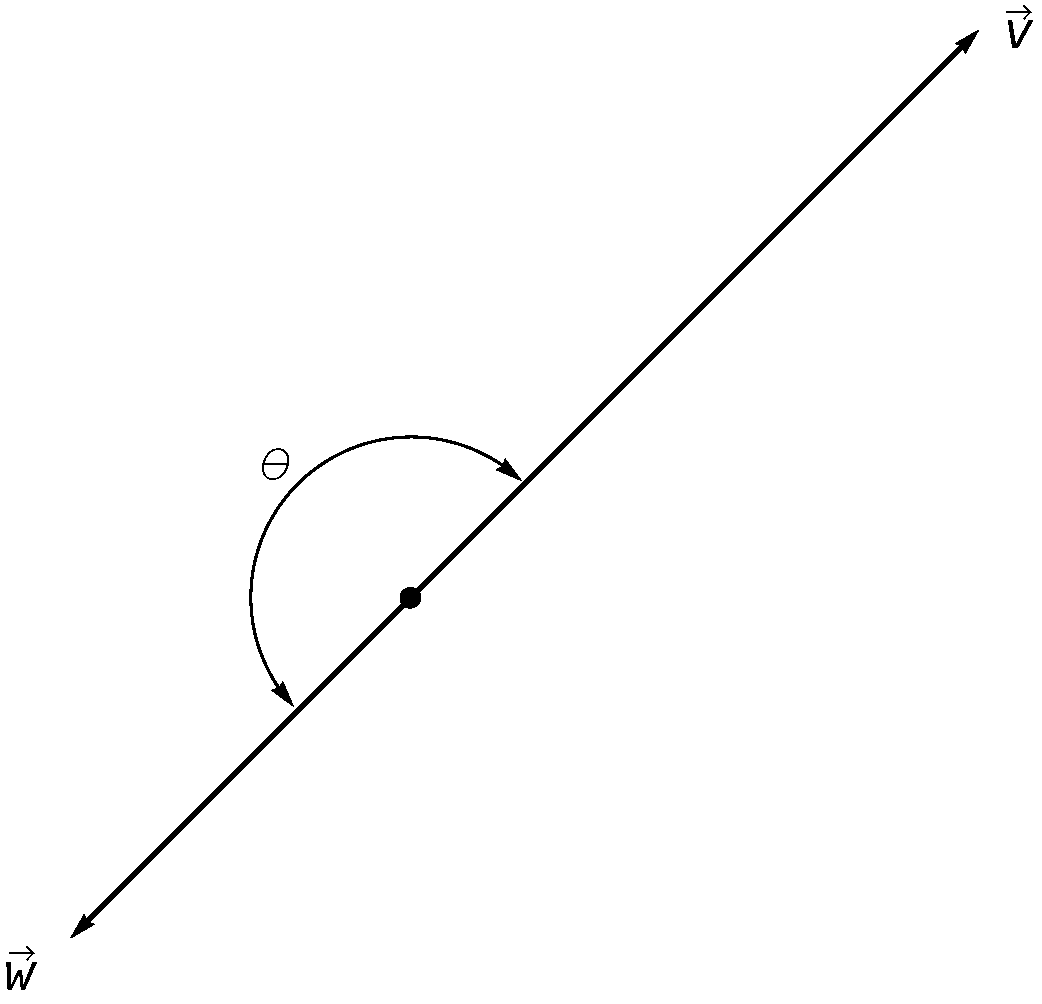
\includegraphics[width=0.3\textwidth]{fig_vector_12c}}
}
\caption{Two vectors $\vec{v}$ and $\vec{w}$ with the same initial point and the angle $\theta$ between them. }
\label{fig_vector_12}
\end{figure}

The following theorem gives us some insight into the geometric role the dot product plays.


\begin{theorem}[Geometric interpretation of dot product] \label{dotproductgeo} 
  If $\vec{v}$ and $\vec{w}$ are nonzero vectors then 
	\begin{equation}
	\vec{v} \cdot \vec{w} = \|\vec{v}\| \|\vec{w}\| \cos(\theta),
	\label{dotproductgeoeq}
	\end{equation}
where $\theta$ is the angle between $\vec{v}$ and $\vec{w}$.  


\end{theorem}
 This theorem states that taking a dot product of two vectors boils down to projecting one vector onto the direction of the second vector and subsequently scaling it with the magnitude of the latter.

% \ifcourse
% \ifanalysis
% 
% We prove this theorem in cases. 
% \begin{itemize}
% \item If $\theta = 0$ (Figure~\ref{fig_vector_13a}), then $\vec{v}$ and $\vec{w}$ have the same direction. It follows that there is a real number $k > 0$ so that $\vec{w} = k \vec{v}$.  Hence, 
% $$\vec{v} \cdot \vec{w} = \vec{v} \cdot (k \vec{v}) = k (\vec{v} \cdot \vec{v}) = k \|\vec{v} \|^2 = k \| \vec{v} \| \|\vec{v}\|.$$
% Since $k > 0$,  $k = |k|$, so $k \|\vec{v}\| = |k| \|\vec{v}\| = \| k \vec{v} \|$.  Hence, 
% $$k \| \vec{v} \| \|\vec{v}\| = \| \vec{v} \| (k\|\vec{v}\|) = \|\vec{v}\| \|k\vec{v}\| = \|\vec{v}\| \|\vec{w}\|.$$
% Since $\cos(0) = 1$, we get  $\vec{v} \cdot \vec{w} = k \| \vec{v}\| \| \vec{v} \| = \|\vec{v} \| \|\vec{w}\|  =  \|\vec{v} \| \|\vec{w}\| \cos(0)$, proving that the formula holds for $\theta = 0$.  

% \item If $\theta = \pi$,  we repeat the argument with the difference being $\vec{w} = k \vec{v}$ where $k < 0$.  In this case, $|k| = -k$, so $k\|\vec{v}\| = -|k| \| \vec{v}\| = -\|k\vec{v}\| = -\| \vec{w}\|$.  Since $\cos(\pi) = -1$, we get 
% $$\vec{v} \cdot \vec{w} = -\|\vec{v}\| \|\vec{w} \| = \|\vec{v}\| \|\vec{w}\| \cos(\pi),$$
% as required. 

% \item Next, if $0 < \theta < \pi$ (Figure~\ref{fig_vector_13b}), the  vectors $\vec{v}$, $\vec{w}$ and $\vec{v} - \vec{w}$ determine a triangle with side lengths $\| \vec{v} \|$, $\| \vec{w} \|$ and $\| \vec{v} - \vec{w} \|$, respectively, as seen below. The law of cosines yields 
% $$\| \vec{v} - \vec{w} \|^2 = \|\vec{v}\|^2 + \|\vec{w}\|^2 - 2\|\vec{v}\| \|\vec{w}\| \cos(\theta).$$
% From Example~\ref{dotprodpropex}, we know $\|\vec{v} - \vec{w}\|^2 = \|\vec{v}\|^2  -2 (\vec{v} \cdot \vec{w}) + \|\vec{w}\|^2$.  Equating these two expressions for $\| \vec{v} - \vec{w} \|^2$ gives 
% $$\|\vec{v}\|^2 + \|\vec{w}\|^2 - 2\|\vec{v}\| \|\vec{w}\| \cos(\theta)  =  \|\vec{v}\|^2  -2 (\vec{v} \cdot \vec{w}) + \|\vec{w}\|^2,$$
% which reduces to 
% $$- 2\|\vec{v}\| \|\vec{w}\| \cos(\theta) =   -2 (\vec{v} \cdot \vec{w}),$$
% or 
% $$\vec{v} \cdot \vec{w} = \|\vec{v}\| \|\vec{w}\| \cos(\theta),$$
% as required. 
% \end{itemize}

% 
% \fi
% \fi


An immediate consequence of Theorem \ref{dotproductgeo} is the following.


\begin{theorem}[Angle between vectors]\label{anglebetweenvectorthm} 
Let $\vec{v}$ and $\vec{w}$ be nonzero vectors and let $\theta$ the angle between $\vec{v}$ and $\vec{w}$.  Then 

\begin{equation}
\theta = \arccos\left( \dfrac{\vec{v} \cdot \vec{w}}{\| \vec{v} \| \|\vec{w} \|}\right) = \arccos(\hat{v} \cdot \hat{w}). 
\label{anglebetweenvectorthmeq}
\end{equation}
\end{theorem}

\begin{proof}
We arrive at Equation~\eqref{anglebetweenvectorthmeq} by solving Equation~\eqref{dotproductgeoeq} for $\theta$.  Since $\vec{v}$ and $\vec{w}$ are nonzero, so are $\| \vec{v} \|$ and $\|\vec{w}\|$.  Hence, we may divide both sides of $\vec{v} \cdot \vec{w} = \| \vec{v} \| \|\vec{w} \| \cos(\theta)$ by $\| \vec{v} \| \|\vec{w} \|$.  Since $0 \leq \theta \leq \pi$ by definition, the values of $\theta$ exactly match the range of the arccosine function, so we get Equation~\eqref{anglebetweenvectorthmeq}.   We can rewrite the argument of the arccosine function as
$$ \frac{\vec{v} \cdot \vec{w}}{\| \vec{v} \| \|\vec{w} \|} = \left(\frac{1}{\|\vec{v}\|} \vec{v}\right) \cdot \left(\frac{1}{\|\vec{w}\|} \vec{w}\right) = \hat{v} \cdot \hat{w},$$
giving us the alternative formula $\theta = \arccos(\hat{v} \cdot \hat{w})$.  
\end{proof}

\begin{example} \label{anglebetweenvectorex}  Find the angle between the following pairs of vectors.
\begin{multicols}{2}
\begin{enumerate}

\item  $\vec{v} = \left( 3, -3\sqrt{3} \right)$ and $\vec{w} = \left(-\sqrt{3}, 1 \right)$

\item  $\vec{v} = \left( 2, 2 \right)$ and $\vec{w} = \left(5, -5\right)$

\end{enumerate}
\end{multicols}

\xhrulefill{gray}{2.5pt}Solution \xhrulefill{gray}{2.5pt}

We use Equation~\eqref{anglebetweenvectorthmeq} in each case below.

\begin{enumerate}

\item  We have $\vec{v} \cdot \vec{w} = \left( 3, -3\sqrt{3} \right) \cdot \left(-\sqrt{3}, 1 \right) = -3\sqrt{3} - 3\sqrt{3} = -6\sqrt{3}$.  As $\| \vec{v} \| = \sqrt{3^2+(-3\sqrt{3})^2}  =6$ and $\| \vec{w}\| = \sqrt{(-\sqrt{3})^2+1^2} = \sqrt{4} =2$,  we find that 
$$
\theta = \arccos\left(\frac{-6\sqrt{3}}{12}\right) = \arccos\left(-\frac{\sqrt{3}}{2}\right) = \frac{5\pi}{6}\,.
$$

\item  For $\vec{v} = \left( 2, 2 \right)$  and $\vec{w} = \left(5, -5\right)$, we find $\vec{v} \cdot \vec{w} = \left( 2, 2 \right) \cdot \left(5, -5\right) = 10-10 = 0$.  Hence, it does not matter what $\| \vec{v} \|$ and $\| \vec{w} \|$ are, and 
$$
\theta = \arccos\left( \frac{\vec{v} \cdot \vec{w}}{\| \vec{v} \| \|\vec{w} \|}\right) = \arccos(0) = \frac{\pi}{2}\,.
$$

\end{enumerate}
\end{example}

Note that the vectors $\vec{v} = \left( 2, 2 \right)$, and $\vec{w} = \left(5, -5\right)$ in Example \ref{anglebetweenvectorex} are called \textbf{orthogonal} (\textit{orthogonaal})\index{vector ! orthogonal vectors}\index{orthogonal vectors}\index[aut]{vector ! orthogonaal} and we write $\vec{v} \perp \vec{w}$, because the angle between them is $\frac{\pi}{2} \mbox{ radians} = 90^{\circ}$.  Geometrically this means that when orthogonal vectors are sketched with the same initial point, the lines containing the vectors are perpendicular.  We state the relationship between orthogonal vectors and their dot product in the following theorem.

\begin{theorem}[Orthogonality of vectors] \label{dotprodorththm} 
  Let $\vec{v}$ and $\vec{w}$ be nonzero vectors.  Then $\vec{v} \perp \vec{w}$ if and only if $\vec{v} \cdot \vec{w} = 0$. \index{ orthogonality} \index[aut]{orthogonaliteit} 

\end{theorem}

\ifcourse
\ifanalysis

\begin{proof}
To prove this theorem, we first assume $\vec{v}$ and $\vec{w}$ are nonzero vectors with  $\vec{v} \perp \vec{w}$.  By definition, the angle between $\vec{v}$ and $\vec{w}$ is $\frac{\pi}{2}$.  By Theorem \ref{dotproductgeo}, it holds that $\vec{v} \cdot \vec{w} = \| \vec{v} \| \| \vec{w} \| \cos\left(\frac{\pi}{2}\right) = 0$. Conversely, if $\vec{v}$ and $\vec{w}$ are nonzero vectors and $\vec{v} \cdot \vec{w} = 0$,  then Theorem \ref{anglebetweenvectorthm} gives 
$$\theta = \arccos\left( \frac{\vec{v} \cdot \vec{w}}{\| \vec{v} \| \|\vec{w} \|}\right) = \arccos\left( \frac{0}{\| \vec{v} \| \|\vec{w} \|}\right) = \arccos(0) = \frac{\pi}{2}\,,$$
so $\vec{v} \perp \vec{w}\,.$  
\end{proof}

\fi
\fi


%\ifcourse
%An important construction is illustrated in Figure~\ref{fig_vector_14}, where vectors $\vec u$ and $\vec v$ are sketched. In Figure~\ref{fig_vector_14a}, a dashed line is drawn from the tip of $\vec u$ to the line containing $\vec v$, where the dashed line is orthogonal to $\vec v$. In Figure~\ref{fig_vector_14b}, the dashed line is replaced with the vector $\vec z$ and  $\vec w$ is formed, parallel to $\vec v$. It is clear by the diagram that $\vec u = \vec w+\vec z$. What is important about this construction is this: $\vec u$ is decomposed as the sum of two vectors, one of which is parallel to $\vec v$ and one that is perpendicular to $\vec v$. 
%
%\begin{figure}
%\centering
%%\right)isebox{0.5cm}{
%\centerline{
%\subfigure[\label{fig_vector_14a}]{\includegraphics[width=0.3\textwidth]{fig_vector_14a}}
%\hspace{0.1cm}
%\subfigure[\label{fig_vector_14b}]{\includegraphics[width=0.3\textwidth]{fig_vector_14b}}
%}
%\caption{Developing the construction of the orthogonal projection. }
%\label{fig_vector_14}
%\end{figure}
%
%The vectors $\vec w$, $\vec z$ and $\vec u$ as shown in Figure \ref{fig_vector_14b} form a right triangle, where the angle between $\vec v$ and $\vec u$ is labelled $\theta$. We can find $\vec w$ in terms of $\vec v$ and $\vec u$.
%
%Using trigonometry, we can state that 
%\begin{equation}
%\norm{\vec w} = \norm{\vec u}\cos(\theta). \label{eq:proj1}
%\end{equation}
%
%
%We also know that $\vec w$ is parallel to to $\vec v$\,; that is, the direction of $\vec w$ is the direction of $\vec v$, described by the unit vector $\vec v/\norm{\vec v}$. The vector $\vec w$ is the vector in the direction $\vec v/\norm{\vec v}$ with magnitude $\norm{\vec u}\cos \theta$:
%
%%\begin{align*}
%%	\vec w &= \Big(\norm{\vec u}\cos(\theta) \Big)\frac{1}{\norm{\vec v}}\vec v.
%%	\intertext{Replace $\cos(\theta)$ using Theorem \ref{dotproductgeo}:}
%%	&= \left(\norm{\vec u}\frac{\vec u \cdot\vec v}{\norm{\vec u}\norm{\vec v}}\right)\frac{1}{\norm{\vec v}} \vec v\\ 
%%	&= \frac{\vec u\cdot \vec v}{\norm{\vec v}^2}\vec v.
%%	\intertext{Now use the properties of the dot product.}
%%	&= \frac{\vec u\cdot\vec v}{\vec v \cdot \vec v}\vec v.
%%\end{align*}
%
%\renewcommand{\arraystretch}{2.5}%
%\[ \begin{array}{rcll}
%\vec w &=& \left(\,\norm{\vec u}\cos(\theta) \right)\dfrac{1}{\norm{\vec v}}\vec v&\\
%			&=& \left(\norm{\vec u}\dfrac{\vec u \cdot\vec v}{\norm{\vec u}\norm{\vec v}}\right)\dfrac{1}{\norm{\vec v}} \vec v&\quad\text{(Replace $\cos(\theta)$ using Theorem \ref{dotproductgeo}.)}\\
%			&=& \dfrac{\vec u\cdot \vec v}{\norm{\vec v}^2}\vec v&\\
%			&=& \dfrac{\vec u\cdot\vec v}{\vec v \cdot \vec v}\vec v.&\quad\text{(Properties of the dot product.)}
%\end{array} \]
%
%
%Since this construction is so important, it is given a special name.
%
%\begin{definition}[Orthogonal projection]\label{def:orthogonal_projection}
%Let nonzero vectors $\vec u$ and $\vec v$ be given. The \textbf{orthogonal projection} (\textit{loodrechte projectie}) of $\vec u$ onto $\vec v$, denoted \textbf{$\proj uv$}, is 
%\index{orthogonal projection}\index{vector ! orthogonal projection}\index[aut]{loodrechte projectie} \index[aut]{vector ! loodrechte projectie}
%$$\proj uv = \frac{\dotp uv}{\dotp vv}\vec v.$$
%
%\end{definition}
%
%\begin{example}\label{ex_dotp4}
%Let $\vec u= \left( -2,1\right)$ and $\vec v=\left( 3,1\right)$. Find $\proj uv$, and sketch all three vectors with initial points at the origin.
%
%\xhrulefill{gray}{2.5pt}Solution \xhrulefill{gray}{2.5pt}
%
%Applying Definition~\ref{def:orthogonal_projection}, we have
%	\begin{align*}
%	\proj uv &= \frac{\dotp uv}{\dotp vv}\vec v \\
%					&= \frac{-5}{10}\left( 3,1\right)\\
%					&= \left( -\frac32,-\frac12\right).
%	\end{align*}
%	Vectors $\vec u$, $\vec v$ and $\proj uv$ are sketched in Figure~\ref{fig_vector_15}. Note how the projection is parallel to $\vec v$; that is, it lies on the same line through the origin as $\vec v$, although it points in the opposite direction. That is because the angle between $\vec u$ and $\vec v$ is obtuse (i.e., greater than $90^\circ$).
%	
%	\begin{figure}[H]
%	\begin{center}
%			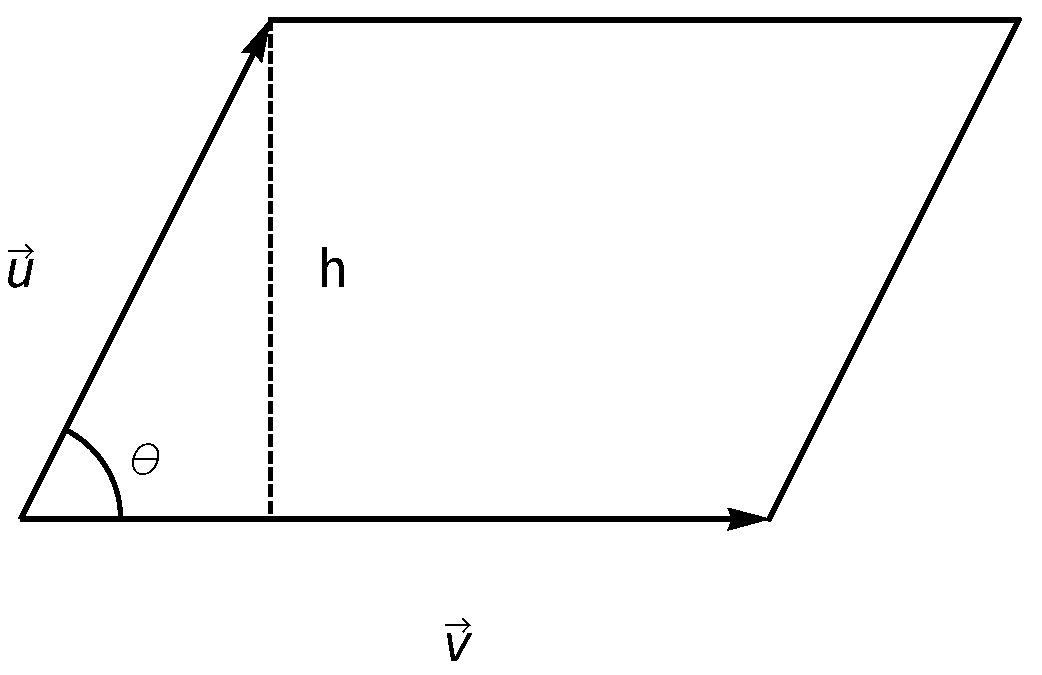
\includegraphics[width=0.45\textwidth]{fig_vector_15}
%	\caption{Graphing the vectors used in Example~\ref{ex_dotp4}. }
%	\label{fig_vector_15}
%	\end{center}
%\end{figure}
%
%\end{example}
%
%
%We can use the properties of the dot product to rearrange the formula found in Definition \ref{def:orthogonal_projection}:
%\begin{align*}
%\proj uv &= \frac{\dotp uv}{\dotp vv}\vec v\\
%		&= \frac{\dotp uv}{\norm{\vec v}^2}\vec v\\
%		&= \left(\vec u \cdot \frac{\vec v}{\norm{\vec v}}\right) \frac{\vec v}{\norm{\vec v}}.
%\end{align*}
%
%The above formula shows that the orthogonal projection of $\vec u$ onto $\vec v$ is only concerned with the direction of $\vec v$, as both instances of $\vec v$ in the formula come in the form $\vec v/\norm{\vec v}$, the unit vector in the direction of $\vec v$.
%
%A special case of orthogonal projection occurs when $\vec v$ is a unit vector. In this situation, the formula for the orthogonal projection of a vector $\vec u$ onto $\vec v$ reduces to just $\proj uv = (\vec u\cdot\vec v)\vec v$, as $\vec v\cdot\vec v = 1$.
%
%This gives us a new understanding of the dot product. When $\vec v$ is a unit vector, essentially providing only direction information, the dot product of $\vec u$ and $\vec v$ gives how much of $\vec u$ is in the direction of $\vec v$. Moreover, when $\vec v$ and $\vec w$ are non-unit vectors, taking a dot product of the two vectors boils down to projecting one vector onto the direction of the second and subsequently scaling it with the magnitude of the latter.
%
%
%\fi



\ifcourse

\ifcalculus
\section{Vectors in three-dimensional space and beyond}
\label{sec_vec_drie_dim}
\fi
\ifanalysis
\section{Vectors in $n$-dimensional space}
\label{sec_vec_n_dim}
\fi
Vectors are of course not limited to the plane as most processes involving forces happen in three-dimensional space. For that reason, we will move our mathematics out of the plane and into space. That is, we begin to think mathematically not only in two dimensions, but in three, and even more. With this foundation, we can explore vectors  in space. 


\subsection{Cartesian coordinates and distance in space}
Up to this point  we have considered mathematics in a two--dimensional world. We have plotted graphs on the $xy$-plane using rectangular and polar coordinates and found the area of regions in the plane. Here, we introduce Cartesian coordinates in space.

Each point $P$ in space can be represented with an ordered triple, $P=(x,y,z)$, where $x$, $y$ and $z$ represent the relative position of $P$ along the $x$-, $y$- and $z$-axes, respectively. Each axis is perpendicular to the other two. For plotting shapes in space a first convention is that the axes must conform to the \textbf{right hand rule} (\textit{rechterhandregel}). This rule states that when the index finger of the right hand is extended in the direction of the positive $x$-axis, and the middle finger (bent inward so it is perpendicular to the palm) points along the positive $y$-axis, then the extended thumb will point in the direction of the positive $z$-axis (Figure~\ref{fig_vector_13}). \index{right hand rule}\index[aut]{rechterhandregel}

	\begin{figure}[h]
	\begin{center}
			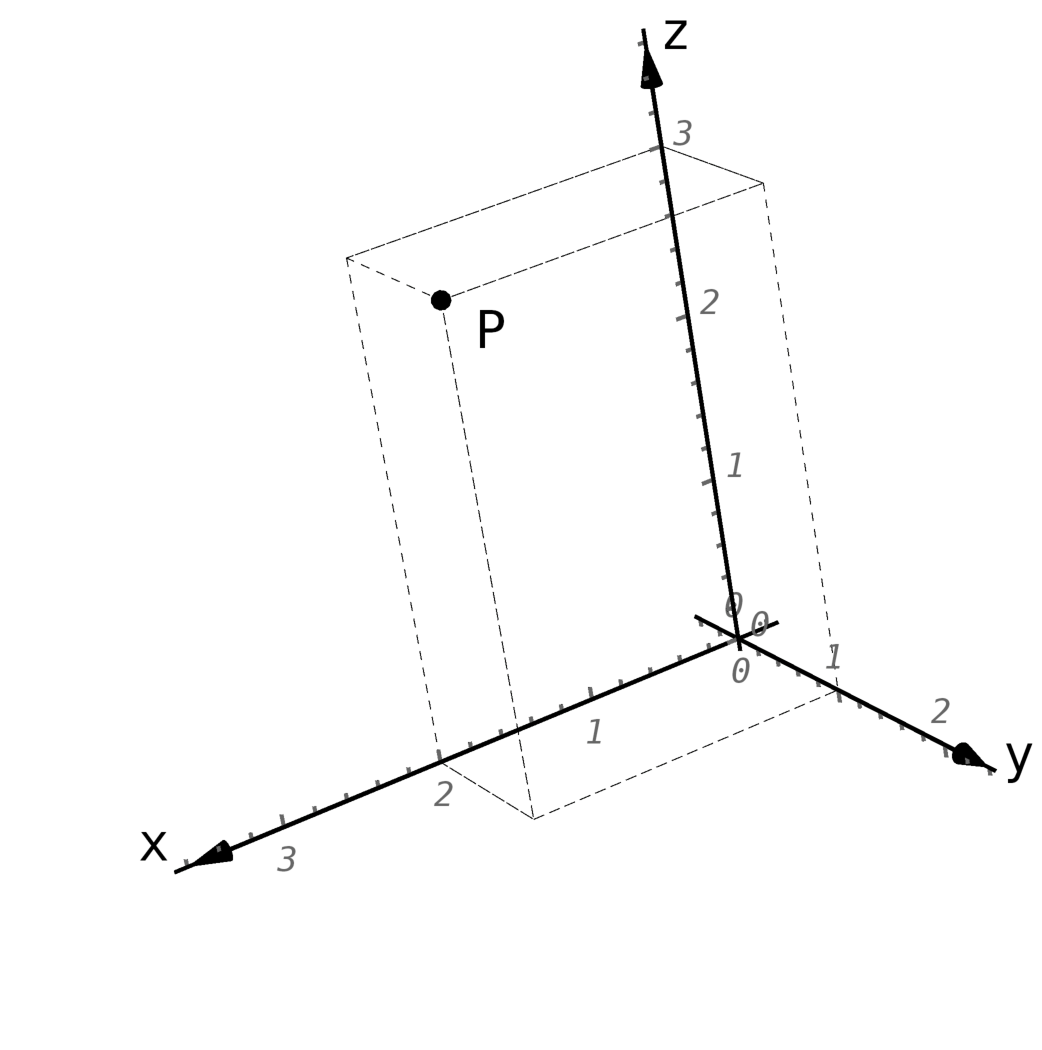
\includegraphics[width=0.35\textwidth]{fig_vector_13}
	\caption{Plotting the point $P=(2,1,3)$ in space. }
	\label{fig_vector_13}
	\end{center}
\end{figure}

As long as the coordinate axes are positioned so that they follow this rule, it does not matter how the axes are drawn on paper. Throughout this text we will adhere to the convention with $xy$-plane as being a horizontal plane, where the positive $z$-axis is pointing up. This point of view is preferred by most mathematicians. Just as the $x$- and $y$-axes divide the plane into four quadrants, the $x$-, $y$-, and $z$-coordinate planes divide space into eight \textbf{octants} (\textit{octant}).  The octant in which $x$, $y$, and $z$ are positive is called the first octant.  The Euclidean distance between two points $P\left(x, y,z\right)$ and  $Q\left(\widetilde{x}, \widetilde{y},\widetilde{z}\right)$ in such a three-dimensional space is given by 
\begin{equation}
d(P,Q)=\sqrt{\left(x-\widetilde{x}\right)^2+\left(y-\widetilde{y}\right)^2+\left(z-\widetilde{z}\right)^2}\,.
\label{def:space_distance}
\end{equation}



\index{octant}\index[aut]{octant}



\ifanalysis

Even though it becomes more difficult to present graphically, it is mathematically of course possible to extend the notion of space to $n$ dimensions. Essentially, a point $P$ in $n$-dimensional space can then be represented in rectangular coordinates by the $n$-tuple $(x_1,x_2,\ldots,x_n)$ using $n$ mutually perpendicular axes. The Euclidean distance between two points $P\left(x_{1}, x_{2},\ldots, x_{n}\right)$ and $Q\left(\widetilde{x}_{1}, \widetilde{x}_{2},\ldots, \widetilde{x}_{n}\right)$ in $n$-dimensional space is given by 
\begin{equation}
d(P,Q)=\sqrt{\left(x_1-\widetilde{x}_1\right)^2+\left(x_2-\widetilde{x}_2\right)^2+\ldots+\left(x_n-\widetilde{x}_n\right)^2}\,.\label{def:space_distancend}
\end{equation}

\fi

\begin{remark}[Higher-dimensional mathematics in art]
The concept of four-dimensional space and the difficulties involved in trying to visualize it helped inspire many modern artists in the first half of the twentieth century, such as Picasso and Weber. The former got introduced to the topic through Poincar\'e's \textit{Elementary Treatise on the Geometry of Four Dimensions}. He incorporated some aspects of four-dimensional mathematics in his painting \textit{Portrait of Daniel-Henry Kahnweiler} (Figure~\ref{fig_vector_14}). 

	\begin{figure}[H]
	\begin{center}
			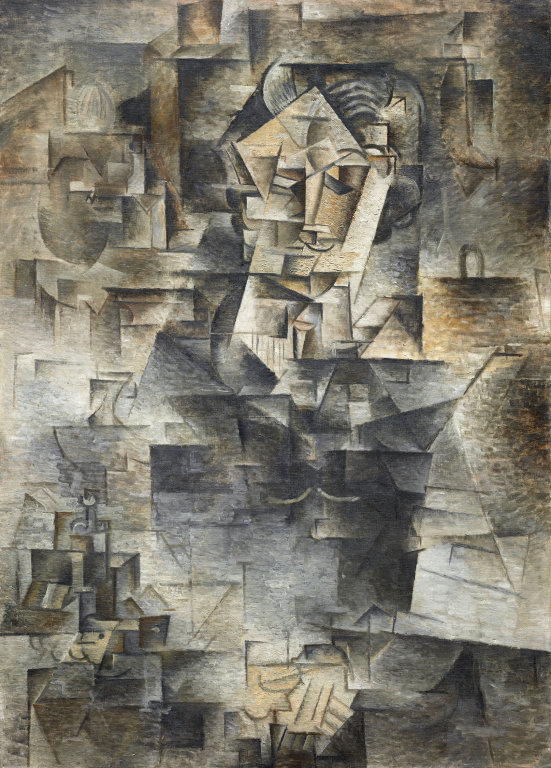
\includegraphics[width=0.3\textwidth]{fig_vector_14}
	\caption{Picasso's portrait of Daniel-Henry Kahnweiler.}
	\label{fig_vector_14}
	\end{center}
\end{figure}

\end{remark}
\subsection{Vector representation and operations in space}
Essentially, all of the definitions and vector operations we introduced in Sections~\ref{sec_vect_repre} and \ref{sec_vector_arith} may be generalized intuitively to three or more dimensions.

\ifcalculus
For instance, in three dimensions the component form of a vector is defined as follows. 
\begin{definition}[Component form of a vector in three dimensions] \label{componentformvector3d}  Suppose $\vec{v}$ is represented by a directed line segment with initial point $P\left(x_0, y_0,z_0\right)$ and terminal point $Q\left(x_1, y_1,z_1\right)$.  The component form of $\vec{v}$ is given by 
\[ \vec{v} = \overrightarrow{PQ} = \left( x_1 - x_0, y_1 - y_0, z_1-z_0 \right). \]


\end{definition}

Likewise, vector addition, scalar multiplication and the dot product, as well as their corresponding properties, generalize naturally to three dimensions.

\begin{definition}[Vector addition in three dimensions] \label{vectoradd3d} 
 Suppose $\vec{v} = \left(v_1,v_2,v_3\right)$ and $\vec{w} = \left(w_1,w_2,w_3\right)$.  The vector $\vec{v} + \vec{w}$ is defined by \index{vector ! addition}\index[aut]{vector ! som}
\[ \vec{v} + \vec{w}  = \left( v_1 + w_1, v_2 + w_2, v_3+ w_3\right). \]


\end{definition}

\pagebreak

\begin{definition}[Scalar multiplication in three dimensions] \label{scalarmultvector3d} \index{vector ! scalar multiplication} \index{scalar multiplication}\index[aut]{vector ! scalaire vermenigvuldiging} \index[aut]{scalaire vermenigvuldiging} If $k$ is a real number and $\vec{v} = \left(v_1,v_2,v_3\right)$, we define $k\vec{v}$ by 
\[k\vec{v} = k\left(v_1,v_2,v_3\right) =\left(k v_1,k v_2, k v_3\right). \]

\end{definition}


\begin{definition}[Dot product in three dimensions] \label{dotproductdefnnd}    
Suppose $\vec{v}$ and $\vec{w}$ are vectors whose component forms are $\vec{v} = \left(v_1,v_2,v_3\right)$ and $\vec{w} = \left(w_1,w_2,w_3\right)$.  The dot product\index{vector ! dot product}\index{vector ! scalar product}\index{dot product}\index[aut]{scalair product}\index[aut]{inproduct} \index[aut]{vector ! scalair product}\index[aut]{vector ! inproduct}  of $\vec{v}$ and $\vec{w}$ is given by
\[ \vec{v} \cdot \vec{w} = \left(v_1,v_2,v_3\right) \cdot \left(w_1,w_2,w_3\right) = v_1w_1 + v_2w_2 + v_3w_3. \]

\end{definition}


Besides, in three dimensions, we can define three principal unit vectors, which make up a standard basis. 
\index{vector ! principal unit vectors} \index[aut]{basisvector}

\begin{itemize}

\item The vector $\hat{\imath} = \left(1,0,0\right)$

\item The vector $\hat{\jmath} = \left(0,1,0\right)$

\item The vector $\hat{k} = \left(0,0,1\right)$

\end{itemize}


\fi 


\ifanalysis

In $n$ dimensions the component form of a vector is defined as follosws. 
\begin{definition}[Component form of a vector in $n$ dimensions] \label{componentformvectornd}  Suppose $\vec{v}$ is represented by a directed line segment with initial point $P\left(x_{1}, x_{2},\ldots, x_{n}\right)$ and terminal point $Q\left(\widetilde{x}_{1}, \widetilde{x}_{2},\ldots, \widetilde{x}_{n}\right)$.  The component form of $\vec{v}$ is given by 

\[ \vec{v} = \overrightarrow{PQ} = \left(\widetilde{x}_1- x_1 , \widetilde{x}_2-x_2, \ldots, \widetilde{x}_n-x_n \right). \]


\end{definition}

Likewise, vector addition, scalar multiplication and the dot product, as well as their corresponding properties, generalize naturally to $n$ dimensions.

\begin{definition}[Vector addition in $n$ dimensions] \label{vectoraddnd} 
 Suppose $\vec{v} = \left(v_1,v_2,\ldots,v_n\right)$ and $\vec{w} = \left(w_1,w_2,\ldots,w_n\right)$.  The vector $\vec{v} + \vec{w}$ is defined by \index{vector ! addition}\index[aut]{vector ! som}

\[ \vec{v} + \vec{w}  = \left( v_1 + w_1, v_2 + w_2, \ldots, v_n+ w_n\right). \]


\end{definition}


\begin{definition}[Scalar multiplication in $n$ dimensions] \label{scalarmultvectornd} \index{vector ! scalar multiplication} \index{scalar multiplication}\index[aut]{vector ! scalaire vermenigvuldiging} \index[aut]{scalaire vermenigvuldiging} If $k$ is a real number and $\vec{v} = \left(v_1,v_2,\ldots,v_n\right)$, we define $k\vec{v}$ by 
\[k\vec{v} = k\left(v_1,v_2,\ldots,v_n\right) =\left(k v_1,k v_2, \ldots, k v_n\right). \]

\end{definition}


\begin{definition}[Dot product in $n$ dimensions] \label{dotproductdefnnd}    
Suppose $\vec{v}$ and $\vec{w}$ are vectors whose component forms are $\vec{v} = \left(v_1,v_2,\ldots, v_n\right)$ and\\  $\vec{w} = \left(w_1,w_2,\ldots,w_n\right)$.  The dot product\index{vector ! dot product}\index{vector ! scalar product}\index{dot product}\index[aut]{scalair product}\index[aut]{inproduct} \index[aut]{vector ! scalair product}\index[aut]{vector ! inproduct}  of $\vec{v}$ and $\vec{w}$ is given by

\[ \vec{v} \cdot \vec{w} = \left(v_1,v_2,\ldots,v_n\right) \cdot \left(w_1,w_2,\ldots,w_n\right) = v_1w_1 + v_2w_2 +\cdots+ v_nw_n. \]

\end{definition}


Besides, in $n$ dimensions, we can define $n$ principal unit vectors $\hat{e}_1$, $\hat{e}_2$, \ldots, $\hat{e}_n$, which make up a standard basis. All components of the $i$-th such principal unit vector are zero, expect the $i$-th component, which is 1. For instance, $\hat{e}_2 = \left(0,1,0,\ldots,0\right)$ or $\hat{e}_n = \left(0,0,0,\ldots,1\right)$.


\index{vector ! principal unit vectors} \index[aut]{basisvector}


\fi 

\begin{example}
Given $\vec{v} = \left(1,2,2\right)$ and $\vec{w} = \left(-1,0,3\right)$, find
\begin{enumerate}
\item The unit vector in the direction of $\vec{v}$.
\item $\vec{v}\cdot\vec{w}$.
\end{enumerate}

\xhrulefill{gray}{2.5pt}Solution \xhrulefill{gray}{2.5pt}

\begin{enumerate}
	\item		We find $\norm{\vec v} = 3$, so the unit vector $\vec z$ in the direction of $\vec v$ is
	$$\hat{z} = \frac13\vec v = \left( \frac13,\frac23,\frac23\right).$$
	\item Using Definition~\ref{dotproductdefnnd} we immediately find
	$$
	\vec{v}\cdot\vec{w}=1(-1)+2(0)+2(3)=5.
	$$
	\end{enumerate}
\end{example}


\begin{example}
Let $\vec u = \left( 1,1,1\right)$, $\vec v = \left( -1,3,-2\right)$ and $\vec w = \left( -5,1,4\right)$. Find the angle between each pair of vectors.


\xhrulefill{gray}{2.5pt}Solution \xhrulefill{gray}{2.5pt}


For this purpose, we use Equation~\eqref{anglebetweenvectorthmeq}. 
\begin{enumerate}
	\item Between $\vec u$ and $\vec v$:
	\begin{align*}
	\theta &= \arccos\left(\frac{\dotp uv}{\norm{\vec u} \, \norm{\vec v}}\right)\\
					&= \arccos\left(\frac{0}{\sqrt{3}\sqrt{14}}\right)\\
					&= \frac{\pi}2.
	\end{align*}
	\item	Between $\vec u$ and $\vec w$:
	\begin{align*}
	\theta &= \arccos\left(\frac{\dotp uw}{\norm{\vec u} \, \norm{\vec w}}\right)\\
					&= \arccos\left(\frac{0}{\sqrt{3}\sqrt{42}}\right)\\
					&= \frac{\pi}2.
	\end{align*}
	\item	Between $\vec v$ and $\vec w$:
	\begin{align*}
	\theta &= \arccos\left(\frac{\dotp vw}{\norm{\vec v} \, \norm{\vec w}}\right)\\
					&= \arccos\left(\frac{0}{\sqrt{14}\sqrt{42}}\right)\\
					&= \frac{\pi}2.
	\end{align*}
\end{enumerate}
\end{example}

\ifanalysis

%http://math.wikia.com/wiki/Proof_of_the_Cauchy-Schwarz_inequality
For $n$-dimensional vectors we have the following important theorem. 
\begin{theorem}[Cauchy-Schwartz inequality]\label{theo:cuachy}
If $\vec{u}$ and $\vec{v}$ are vectors in $\mathbb{R}^n$, then
$$|\vec{u}\cdot\vec{v}|\le\|\vec{u}\| \, \|\vec{v}\|$$
\end{theorem}
% This can be proofed by resorting to our insight into the solutions of quadratic equations.

% If either $\vec{u}$ or $\vec{v}$ are the zero vector, the statement holds trivially, so assume that both vectors are non-zero. Let $r$ be a scalar and $\vec{w}=r\vec{u}+\vec{v}$. Since, for any non-zero vector $\vec{u}$, it holds that $\vec{u}\cdot\vec{u}=\vec{u}^2\geq0$, we have that 
% \begin{align} 
% 0&\le(r\vec{u}+\vec{v})\cdot(r\vec{u}+\vec{v})\\ 0&\le r^2(\vec{u}\cdot\vec{u})+2r(\vec{u}\cdot\vec{v})+(\vec{v}\cdot\vec{v})\\ 0&\le ar^2+2br+c \,,
% \end{align}
% where $a=\vec{u}\cdot\vec{u}$, $b=\vec{u}\cdot\vec{v}$ and $c=\vec{v}\cdot\vec{v}$. It can be seen clearly that $p(r)=ar^2+2br+c$ is a quadratic polynomial that is non-negative for any $r$. Consequently, the polynomial has two complex roots, or has a single distinct real root. More precisely, since its roots are given by
% $$
% \frac{-2b\pm\sqrt{4b^2-4ac}}{2a}=-b\pm\sqrt{b^2-ac}
% $$
% the term $b^2-ac$ must either be negative, yielding two complex roots, or 0, yielding a single real root. Thus 
% \begin{align}
% &b^2-ac\le0\\
% &b^2\le ac\\
% &b\le\sqrt{ac}
% \end{align}
% Substituting the values of $a$, $b$, $c$ into the last of these inequalities, it can be seen that 
% \begin{align} 
% \sqrt{(\vec{u}\cdot\vec{v})^2}&\le\sqrt{\vec{u}\cdot\vec{u}}\,\sqrt{\vec{v}\cdot\vec{v}}\\ |\vec{u}\cdot\vec{v}|&\le\|\vec{u}\| \, \|\vec{v}\| 
% \end{align}

We conclude this section with an example. 

\begin{example}
For any  $x$, $y$ $z\in\mathbb{R}^+$ prove that
$$
\sqrt{x(3x+y)}+\sqrt{y(3y+z)}+\sqrt{z(3z+x)}\leq2(x+y+z)\,.
$$

\xhrulefill{gray}{2.5pt}Solution \xhrulefill{gray}{2.5pt}

By Cauchy-Schwartz we have that
\begin{eqnarray*}
&&\sqrt{x(3x+y)}+\sqrt{y(3y+z)}+\sqrt{z(3z+x)}\\[0.2cm]
&\leq&\sqrt{\left((\sqrt{x})^2+(\sqrt{y})^2+(\sqrt{z})^2\right)\left((\sqrt{3x+y})^2+(\sqrt{3y+z})^2+(\sqrt{3z+x})^2\right)}\\[0.2cm]
&=&\sqrt{4(x+y+z)^2}\\
&=&2(x+y+z)
\end{eqnarray*}
\end{example}

\fi
\fi

\ifcourse


\section{The cross product}
\label{sec:cross_product}
\ifanalysis\subsection{Definition and properties}\fi
Orthogonality is immensely important. A quick scan of your current environment will undoubtedly reveal numerous surfaces and edges that are perpendicular to each other. The dot product provides a quick test for orthogonality:  vectors $\vec u$ and $\vec v$ are perpendicular if and only if, $\dotp uv=0$.




Given two non--parallel, nonzero vectors $\vec u$ and $\vec v$ in space, it is very useful to find a vector $\vec w$ that is perpendicular to both $\vec u$ and $\vec v$. There is a operation, called the cross product, that creates such a vector.

\begin{definition}[Cross product]\label{def:cross_product}
Let $\vec u =\left( u_1,u_2,u_3\right)$ and $\vec v = \left( v_1,v_2,v_3\right)$ be vectors in $\mathbb{R}^3$. The \textbf{cross product} (\textit{kruisproduct of vectorieel product}) of $\vec u$ and $\vec v$, denoted $\crossp uv$, is the vector
\index{vector ! cross product}\index{cross product}\index[aut]{vector ! kruisproduct}\index[aut]{kruisproduct}
$$
\crossp uv = \left( u_2v_3-u_3v_2,-(u_1v_3-u_3v_1),u_1v_2-u_2v_1\right).
$$
\end{definition}

\ifanalysis

The cross product can also be expressed as the formal determinant:
\renewcommand{\arraystretch}{1}
$$
\crossp uv  ={\begin{vmatrix}\hat {i} &\hat {j} &\hat {k} \\u_{1}&u_{2}&u_{3}\\v_{1}&v_{2}&v_{3}\\\end{vmatrix}}\,,
$$
which makes it easier to remember. Using cofactor expansion along the first row, it expands to
$$
{\displaystyle {\begin{aligned}\crossp uv  &={\begin{vmatrix}u_{2}&u_{3}\\v_{2}&v_{3}\end{vmatrix}}\hat {i} -{\begin{vmatrix}u_{1}&u_{3}\\v_{1}&v_{3}\end{vmatrix}}\hat {j} +{\begin{vmatrix}u_{1}&u_{2}\\v_{1}&v_{2}\end{vmatrix}}\hat {k} \\&=(u_{2}v_{3}-u_{3}v_{2})\hat {i} -(u_{1}v_{3}-u_{3}v_{1})\hat {j} +(u_{1}v_{2}-u_{2}v_{1})\hat {k} ,\end{aligned}}}
$$
which gives the components of the resulting vector directly. 


\fi
\begin{example}\label{ex_crossp1}
Let $\vec u = \left( 2,-1,4\right)$ and $\vec v = \left( 3,2,5\right)$. Find $\crossp uv$, and verify that it is orthogonal to both $\vec u$ and $\vec v$.

\pagebreak
\xhrulefill{gray}{2.5pt}Solution \xhrulefill{gray}{2.5pt}

Using Definition~\ref{def:cross_product}, we have
\ifcalculus
$$\crossp uv = \left( (-1)5-(4)2,-\big((2)5-(4)3\big), (2)2-(-1)3\right)= \left( -13,2,7\right).$$ 
\fi
\ifanalysis
\renewcommand{\arraystretch}{1}
$$
{\displaystyle {\begin{aligned}\crossp uv  &=\begin{vmatrix}\hat {i} &\hat {j} &\hat {k} \\2&-1&4\\3&2&5\\\end{vmatrix}\\
&=\left( \big((-1)5-(4)2\big)\hat i,-\big((2)5-(4)3\big)\hat j, \big((2)2-(-1)3\big)\hat k\right)\\
&= \left( -13\hat i,2\hat j,7\hat k\right)\end{aligned}}}
$$
\fi

\enlargethispage{2\baselineskip}
We now test whether or not $\crossp uv$ is orthogonal to $\vec u$ and $\vec v$ using the dot product:
$$\big(\crossp uv\big) \cdot \vec u = \left( -13,2,7\right)\cdot \left( 2,-1,4\right)= 0,$$
$$\big(\crossp uv\big) \cdot \vec v = \left( -13,2,7\right)\cdot \left( 3,2,5 \right)= 0.$$
Since both dot products are zero, $\crossp uv$ is indeed orthogonal to both $\vec u$ and $\vec v$.
\end{example}



Given the vectors  $\vecu$, $\vecv$ and $\vecw$ in $\mathbb{R}^3$ and the scalar $c$, the following  properties hold for the cross product, each of which can be verified by referring to the definition.

\begin{itemize}
	\item   \textbf{Anticommutative property:}
	$$\crossp uv = -(\crossp vu),$$ 
	
	\item      \textbf{Distributive properties:}
	\begin{eqnarray*}
		 (\vec u+\vec v)\times \vecw &=& \crossp uw+\crossp vw,\\[0.2cm]
		\vec u \times (\vec v+\vec w) &=& \crossp uv+\crossp uw,
	\end{eqnarray*}
	
	\item		\textbf{Compatibility with scalar multiplication:}
	$$c(\crossp uv) = (c\vecu) \times \vec v = \vecu \times (c\vecv),$$
	
	\item       \textbf{Orthogonality properties:}
	\begin{eqnarray*}
		(\crossp uv)\cdot \vecu &=& 0,\\ 
		(\crossp uv)\cdot \vecv &=& 0,
	\end{eqnarray*}
	
	\item \textbf{Zero cross product:}
	$$\crossp u0 = \vec 0,$$
	    
	\item \textbf{Self cross product:}
	$$\crossp uu = \vec 0,$$
	
	\item		\textbf{Triple Scalar Product}:
	$$\vecu \cdot (\vecv\times\vecw) = (\crossp uv)\cdot \vecw \,.$$
\end{itemize}


Another wonderful property of the cross product, as defined, is that it follows the right hand rule. Given $\vec u$ and $\vec v$ in $\mathbb{R}^3$ with the same initial point, point the index finger of your right hand in the direction of $\vecu$ and let your middle finger point in the direction of $\vecv$. Your thumb will naturally extend in the direction of $\crossp uv$. If you switch, and point the index finger in the direction of $\vecv$ and the middle finger in the direction of $\vecu$, your thumb will now point in the opposite direction, allowing you to visualize the anticommutative property of the cross product.

The property $\crossp uu = \vec 0$ reveals something more interesting than the cross product of a vector with itself is $\vec 0$. Let $\vec u$ and $\vec v$ be parallel vectors; that is, let there be a scalar $c$ such that $\vecv = c\vecu$. Consider their cross product:
\begin{align*}
\crossp uv &= \vecu \times (c\vec u) \\
					&=	\parbox{50pt}{$c(\crossp uu)$}\\
					&= \parbox{50pt}{$\vec 0$.}
\end{align*}

This hints at something deeper. Theorem~\ref{dotproductgeo} related the angle between two vectors and their dot product; there is a similar relationship relating the cross product of two vectors and the angle between them, given by the following theorem.

\begin{theorem}[The cross product and angles]\label{thm:cross_product}
Let $\vec u$ and $\vec v$ be nonzero vectors in $\mathbb{R}^3$. Then
$$\norm{\crossp uv} = \vnorm u\, \vnorm v \sin (\theta),$$
where $\theta$, $0\leq \theta \leq \pi$, is the angle between $\vecu$ and $\vecv$.
\end{theorem}

Note that this theorem makes a statement about the magnitude of the cross product. When the angle between $\vecu$ and $\vecv$ is 0 or $\pi$ (i.e., the vectors are parallel), the magnitude of the cross product is 0. The only vector with a magnitude of 0 is $\vec 0$, hence the cross product of  parallel vectors is $\vec 0$.

We demonstrate the truth of this theorem in the following example.

\begin{example}\label{ex_crossp3}
Let $\vec u = \left( 1,3,6\right)$ and $\vec v = \left( -1,2,1\right)$. Find the angle between $\vecu$ and $\vecv$, and the magnitude of $\crossp uv$.

\ifanalysis\pagebreak\fi
\xhrulefill{gray}{2.5pt}Solution \xhrulefill{gray}{2.5pt}


We use Theorem \ref{dotproductgeo} to find the angle between $\vecu$ and $\vecv$: 
\begin{align*}
\theta &= \arccos\left(\frac{\dotp uv}{\vnorm u\, \vnorm v}\right) \\
			&= \arccos\left(\frac{11}{\sqrt{46}\sqrt{6}}\right)\\
			&\approx 0.8471 = 48.54^\circ.
\end{align*}

Since $\crossp uv = \left( -9,-7,5\right)$ we have $\norm{\crossp uv} = \sqrt{155}.$ The question now is whether or not \\ $\norm{\crossp uv} = \vnorm u\, \vnorm v\sin(\theta)$? Using numerical approximations, we find:
\begin{align*}
\norm{\crossp uv} &=\sqrt{155}  & \vnorm u\,\vnorm v \sin(\theta) & = \sqrt{46}\sqrt{6}\sin (0.8471)\\
									&\approx 12.45, & &\approx 12.45.
\end{align*}
Numerically, they seem equal. Using a right triangle, one can show that 
$$\sin\left(\arccos\left(\frac{11}{\sqrt{46}\sqrt{6}}\right)\right) = \frac{\sqrt{155}}{\sqrt{46}\sqrt{6}},$$ which allows us to verify Theorem~\ref{thm:cross_product} exactly.
\end{example}




\ifanalysis


It is a standard geometry fact that the area of a parallelogram is $A = bh$, where $b$ is the length of the base and $h$ is the height of the parallelogram. As shown when defining vector addition (Figure~\ref{fig_vector_2}), two vectors $\vecu$ and $\vecv$ define a parallelogram when drawn from the same initial point, as illustrated in Figure \ref{fig_vector_15}. Trigonometry tells us that $h = \vnorm u \sin (\theta)$, hence the area of the parallelogram is 

\begin{equation}
A = \vnorm u\,\vnorm v\sin(\theta) = \norm{\crossp uv},\label{eq:crossp1}
\end{equation}
where the second equality comes from Theorem \ref{thm:cross_product}. We illustrate using Equation~\eqref{eq:crossp1} in the following examples.

	\begin{figure}[h]
	\begin{center}
			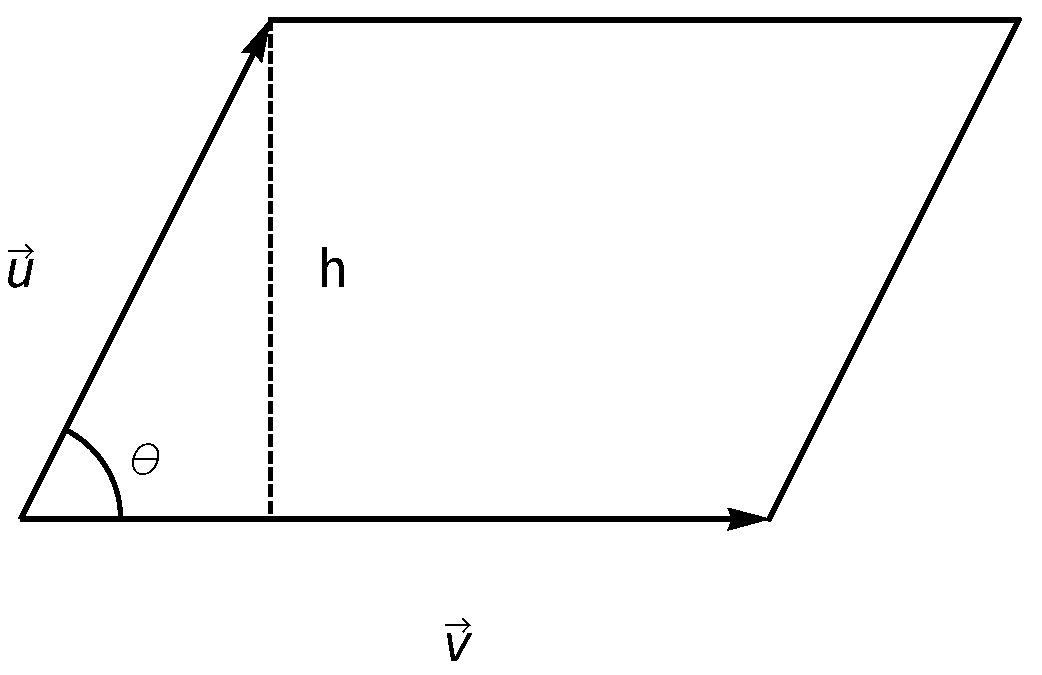
\includegraphics[width=0.35\textwidth]{fig_vector_15}
	\caption{Using the cross product to find the area of a parallelogram.}
	\label{fig_vector_15}
	\end{center}
\end{figure}

\begin{example}\label{ex_crossp4}
\begin{enumerate}
	\item Find the area of the parallelogram defined by the vectors $\vecu = \left( 2,1\right)$ and $\vecv = \left( 1,3\right)$.
	\item	Find the area of the triangle with vertices $A=(1,2)$, $B=(2,3)$ and $C=(3,1)$.
\end{enumerate}

\ifanalysis\pagebreak\fi
\xhrulefill{gray}{2.5pt}Solution \xhrulefill{gray}{2.5pt}


\begin{enumerate}
	\item  We have a slight problem in that our vectors exist in $\mathbb{R}^2$, not $\mathbb{R}^3$, and the cross product is only defined on vectors in $\mathbb{R}^3$. We skirt this issue by viewing $\vec u$ and $\vecv$ as vectors in the $xy$-plane of $\mathbb{R}^3$, and rewrite them as $\vec u = \left( 2,1,0\right)$ and $\vecv =\left( 1,3,0\right)$. We can now compute the cross product. 
	It is easy to show that $\crossp uv = \left( 0,0,5\right)$; therefore the area of the parallelogram is $A = \norm{\crossp uv} = 5$.
	
	\item We can choose any two sides of the triangle to use to form vectors; we choose $\vv{AB} = \left( 1,1\right)$ and $\vv{AC}=\left( 2,-1\right)$. As in the previous example, we will rewrite these vectors with a third component of 0 so that we can apply the cross product. The area of the triangle is
$$\frac12\norm{\vv{AB}\times\vv{AC}} = \frac12\norm{\left( 1,1,0\right)\times \left( 2,-1,0\right)} = \frac12\norm{\left( 0,0,-3\right)} = \frac32.$$

	\end{enumerate}
\end{example}


%The cross product also has many applications in engineering, but here we will focus on its use for computing \textbf{torque} (\textit{moment}). This is a measure of the turning force applied to an object. A classic scenario involving torque is the application of a wrench to a bolt. When we represent the force and wrench with vectors $\vec F$ and $\vec \ell$, we see that the bolt moves (because of the threads) in a  direction orthogonal to $\vec F$ and $\vec \ell$. Torque is usually represented by the Greek letter $\tau$, or tau, and has units of N$\cdot$m, a Newton--meter.\index[aut]{moment}\index{torque}
%
%When a force $\vec F$ is applied to a lever arm $\vec \ell$, the resulting torque is 
%\begin{equation}\vec \tau = \crossp \ell F.\label{eq:crossp3}\end{equation}
%
%
%
%\begin{example}\label{ex_crossp7}
%A lever of length 2 metres makes an angle with the horizontal of $45^\circ$ (Figure~\ref{fig_vector_18}). Find the resulting torque when a force of 10 N is applied to the end of the level where:
%\begin{enumerate}
%	\item the force is perpendicular to the lever, and
%	\item	the force makes an angle of $60^\circ$ with the lever.
%\end{enumerate}
%
%
%	\begin{figure}[H]
%	\begin{center}
%			\includegraphics[width=0.35\textwidth]{fig_vector_18}
%	\caption{Showing a force being applied to a lever in Example \ref{ex_crossp7}.}
%	\label{fig_vector_18}
%	\end{center}
%\end{figure}
%
%
%\xhrulefill{gray}{2.5pt}Solution \xhrulefill{gray}{2.5pt}
%
%\begin{enumerate}
%	\item We start by determining vectors for the force and lever arm. Since the lever arm makes a $45^\circ$ angle with the horizontal and is 2 metres long, we have $\vec \ell = 2\left( \cos 45^\circ,\sin 45^\circ\right)= \left( \sqrt2,\sqrt2\right).$
%	Since the force vector is perpendicular to the lever arm (as seen in the left hand side of Figure \ref{fig_vector_18}),  we can conclude it is making an angle of $-45^\circ$ with the horizontal. As it has a magnitude of 10 N, we can state $\vec F = 10\left( \cos (-45^\circ), \sin(-45^\circ)\right)= \left( 5\sqrt2,-5\sqrt2\right).$
%	
%	Using Equation~\eqref{eq:crossp3} to find the torque requires a cross product. We again let the third component of each vector be 0  and compute the cross product:
%	\begin{align*}
%	\vec\tau &= \crossp \ell F \\
%				&= \left( \sqrt2,\sqrt2,0\right)\times \left( 5\sqrt2,-5\sqrt2,0\right)\\
%				&= \left( 0,0,-20\right).
%	\end{align*}
%	This clearly has a magnitude of 20 Nm.
%	
%	We can view the force and lever arm vectors as lying on the page; our computation of $\vec\tau$ shows that the torque goes into the page. This follows the Right Hand Rule of the cross product, and it also matches well with the example of the wrench turning the bolt. Turning a bolt clockwise moves it in.
%	
%	\item		Our lever arm can still be represented by $\vec \ell = \left( \sqrt2,\sqrt2\right)$. As our force vector makes a $60^\circ$ angle with $\vec \ell$, we can see that $\vec F$ makes a $-15^\circ$ angle with the horizontal. Thus 
%	\begin{align*}
%	\vec F = 10\left( \cos\left(-15^\circ\right),\sin\left(-15^\circ\right)\right)&= \left( \frac{5(1+\sqrt3)}{\sqrt2},\frac{5(-1+\sqrt3)}{\sqrt2}\right)\\
%	&\approx \left( 9.659,-2.588\right).\end{align*}
%	
%	We again make the third component 0 and take the cross product to find the torque:
%	\begin{align*}
%	\vec\tau &= \crossp \ell F\\
%					&= \left( \sqrt2,\sqrt2,0\right)\times  \left( \frac{5(1+\sqrt3)}{\sqrt2},\frac{5(-1+\sqrt3)}{\sqrt2},0\right)\\
%					&= \left( 0,0,-10\sqrt3\right)\\
%					&\approx \left( 0,0,-17.321\right).
%	\end{align*}
%	As one might expect, when the force and lever arm vectors are orthogonal, the magnitude of force is greater than when the vectors are not orthogonal.
%\end{enumerate}
%\end{example}


\fi

\begin{remark}[Computational geometry]
In computational geometry of the plane, the cross product is used to determine the sign of the acute angle defined by three points $\displaystyle P_{1}=(x_{1},y_{1}),P_{2}=(x_{2},y_{2})$,  and  $P_{3}=(x_{3},y_{3})$. It corresponds to the direction (upward or downward) of the cross product of the two vectors defined by the two pairs of points $(P_{1},P_{2})$  and $(P_{1},P_{3})$. The sign of the acute angle is the sign of the expression
$$
{\displaystyle (x_{2}-x_{1})(y_{3}-y_{1})-(y_{2}-y_{1})(x_{3}-x_{1}),} 
$$
which is the signed length of the cross product of the two vectors. If the result is 0, the points are collinear; if it is positive, the three points constitute a positive angle of rotation around  $P_{1}$ from $P_{2}$ to $P_{3}$, otherwise a negative angle.
\end{remark}

\fi


%%%%%%%%%%%%%%%%%%%%%
% Oefeningen cursus
%%%%%%%%%%%%%%%%%%%%%
\ifcourse
\newpage

\section{Exercises}

\renewcommand{\ExerciseListName}{Opgave}
\subsection*{\nameref{sec_vector_arith}}

%%%%%%%%%%%%%%%%%
%Oefening 3
%%%%%%%%%%%%%%%%% 
\begin{Exercise}[difficulty = 1] Draw the vectors 
	\[\vec{a}=(3,-2),\quad \vec{b}=\left(-\dfrac{4}{3},0\right),\quad \vec{c}=(0,2)\quad \text{ en } \quad \vec{d}=(1,-1), \]
	and determine their size and direction.
\end{Exercise}

\setboolean{firstanswerofthechapter}{true}
\begin{Answer}\phantom{}
	    \Question  $\vec{a}=(3,-2) \quad \Rightarrow \quad \norm{\vec a} = \sqrt{13}$ \quad and \quad $ \theta = \arctan\left( - \dfrac{2}{3} \right)$
	    \Question  $\vec{b}=\left(\pi, -\dfrac{4}{3}\right) \quad \Rightarrow \quad \norm{\vec b} = \dfrac{4}{3}$ \quad and \quad $ \theta = \pi$
	    \Question  $\vec{c}=(0,2) \quad \Rightarrow \quad \norm{\vec c} = 2$ \quad and \quad $ \theta = \dfrac{\pi}{2}$
	    \Question  $\vec{d}=(1,-1) \quad \Rightarrow \quad \norm{\vec d} = \sqrt{2}$ \quad and \quad $ \theta = - \dfrac{\pi}{4}$
\end{Answer}
\setboolean{firstanswerofthechapter}{false}

%%%%%%%%%%%%%%%%%
%Oefening 2
%%%%%%%%%%%%%%%%% 
\begin{Exercise} Solve the equations below to $\vec{x}$. What are the coordinates for $\vec{x}$ if $A=(3,2)$ and $B=(1,4)$? 
	\begin{multicols}{2}
	\Question[difficulty = 1] $\vec{a}+\vec{x}+\vec{b}=\vec{0}$
	\Question[difficulty = 1] $\vec{a}-\vec{b}=2\vec{b}+\vec{x}-\vec{a}$ 
	\Question[difficulty = 1] $3\left(\vec{x}-\vec{a}\right)=\vec{x}-\vec{b}$
	\Question[difficulty = 1] $2\left(\vec{x}-\vec{a}\right)=3\bigl(\vec{x}-\vec{b}\bigr)$
	\EndCurrentQuestion
	\end{multicols}

\end{Exercise}

\begin{Answer}\phantom{}
    
	\Question $\vec{a}+\vec{x}+\vec{b}=\vec{o} \quad \Leftrightarrow \quad \vec{x} = -\vec{a}-\vec{b} \quad \Rightarrow \quad \vec{x} = (-4,-6)$  
	\Question $\vec{a}-\vec{b}=2\vec{b}+\vec{x}-\vec{a} \quad \Leftrightarrow \quad \vec{x} = 2\vec{a} - 3 \vec{b} \quad \Rightarrow \quad \vec{x} = (3,-8) $ 
	\Question $3\left(\vec{x}-\vec{a}\right)=\vec{x}-\vec{b} \quad \Leftrightarrow \quad \vec{x} = \dfrac{3 \vec{a} - \vec{b}}{2} \quad \Rightarrow \quad \vec{x} = (4,1)$
	\Question $2\left(\vec{x}-\vec{a}\right)=3\bigl(\vec{x}-\vec{b}\bigr) \quad \Leftrightarrow \quad \vec{x} =  -2\vec{a}+3\vec{b} \quad \Rightarrow \quad \vec{x} = (-3,8) $
\end{Answer}


%%%%%%%%%%%%%%%%%
%Oefening 10 Bio-irs
%%%%%%%%%%%%%%%%% 	
\ifanalysis
\begin{Exercise} Consider $M$ as the center of $[AB]$. Prove that for any point $X$ in the plane, the following holds. %VC Elien, oef 14, hfdstk 2
	\Question[difficulty = 2] $\left(\overrightarrow{AX}\right)^2+\left(\overrightarrow{BX}\right)^2=2\left(\overrightarrow{MX}\right)^2+2\left(\overrightarrow{MB}\right)^2$
	\Question[difficulty = 2] $\left(\overrightarrow{AX}\right)^2-\left(\overrightarrow{BX}\right)^2=2\,\overrightarrow{AB}\, \overrightarrow{MX}$

\end{Exercise}

\begin{Answer}\phantom{}
    Write \ $\overrightarrow{AX}$ \ as \ $\overrightarrow{AM} + \overrightarrow{MX}$ \ and \ $\overrightarrow{BX}$ \ als \ $\overrightarrow{BM} + \overrightarrow{MX}$. \\
    $M$ at the middle of $[AB]: \quad \overrightarrow{AM} = \overrightarrow{MB} = -\overrightarrow{BM} $ \; and \;  $\left(\overrightarrow{AM}\right)^2 = \left(\overrightarrow{BM}\right)^2$
    
	    \Question $\left(\overrightarrow{AX}\right)^2+\left(\overrightarrow{BX}\right)^2 = \left(\overrightarrow{AM}\right)^2 + 2\, \overrightarrow{AM} \cdot \overrightarrow{MX} + \left(\overrightarrow{MX}\right)^2 + \left(\overrightarrow{BM}\right)^2 + 2\, \overrightarrow{BM} \cdot \overrightarrow{MX} + \left(\overrightarrow{MX}\right)^2 $ \\
	    $= 2\, \left(\overrightarrow{BM}\right)^2 + 2\, \left(\overrightarrow{MX}\right)^2 + 2 \, \overrightarrow{BM} \cdot \overrightarrow{MX} - 2\, \overrightarrow{BM} \cdot \overrightarrow{MX} 
	    =2\left(\overrightarrow{MX}\right)^2+2\left(\overrightarrow{MB}\right)^2$
		\Question $\left(\overrightarrow{AX}\right)^2-\left(\overrightarrow{BX}\right)^2 = \left(\overrightarrow{AM}\right)^2 + 2\, \overrightarrow{AM} \cdot \overrightarrow{MX} + \left(\overrightarrow{MX}\right)^2 + \left(\overrightarrow{BM}\right)^2 + 2\, \overrightarrow{BM} \cdot \overrightarrow{MX} + \left(\overrightarrow{MX}\right)^2 $ \\
		$= 2 \left(\overrightarrow{AM} - \overrightarrow{BM} \right) \cdot \overrightarrow{MX} = 2 \left(\overrightarrow{AM} + \overrightarrow{MB} \right) \cdot \overrightarrow{MX}=2\,\overrightarrow{AB}\cdot \overrightarrow{MX}$
    
\end{Answer}
	
%%%%%%%%%%%%%%%%%
%Oefening 11 Bio-irs
%%%%%%%%%%%%%%%%% 
\begin{Exercise}[difficulty = 1] Show that the triangle with vertices $A=(2,1)$, $B=(6,4)$ and $C=(5,-3)$ is isosceles.

\end{Exercise}

\begin{Answer}\phantom{}
    $d(A,B) = d(A,C) = 5$
\end{Answer}
	
%%%%%%%%%%%%%%%%%
%Oefening 12 Bio-irs
%%%%%%%%%%%%%%%%% 
\begin{Exercise}[difficulty = 1] Show that the triangle with vertices  $A=(0,0)$, $B=\left(1,\sqrt{3}\right)$ and $C=(2,0)$ is equilateral.

\end{Exercise}

\begin{Answer}\phantom{}
    $d(A,B) = d(A,C) = d(B,C) = 2$
\end{Answer}
\fi

%%%%%%%%%%%%%%%%%
%Oefening 14 Bio-irs
%%%%%%%%%%%%%%%%% 
\ifanalysis
\begin{Exercise}[difficulty=2] A wind vane mounted on top of a car traveling north at $50$ km/h indicates that the wind is coming from the west. If the car is traveling twice as fast, the wind vane indicates that the wind is coming from the northwest. From which direction is the wind coming and what is its speed? 

\end{Exercise}

\begin{Answer}\phantom{}
    The wind is coming from the southwest and its speed is $50{2}$ km/hr.
\end{Answer}
\fi


\subsection*{\nameref{sec_eenheidsvect}}
%%%%%%%%%%%%%%%%%
%Oefening 1
%%%%%%%%%%%%%%%%% 
\begin{Exercise} Consider the following points: $A=(-1,2),\ B=(2,0),\ C=(1,-3)$ and $D=(0,4)$. Express the vectors below using the basis vectors $\hat{\imath}$ and $\hat{\jmath}$. 
	\begin{multicols}{3}
		\Question[difficulty = 1] $\overrightarrow{AB}$
		\Question[difficulty = 1] $\overrightarrow{BA}$
		\Question[difficulty = 1] $\overrightarrow{AC}$
		\Question[difficulty = 1] $\overrightarrow{AB} - \overrightarrow{BC} $
		\Question[difficulty = 1] $\overrightarrow{AC} - 2 \overrightarrow{AB} + 3 \overrightarrow{CD} $
		\Question[difficulty = 1] $\dfrac{\overrightarrow{AB} + \overrightarrow{AC} + \overrightarrow{AD}}{3}$
        \EndCurrentQuestion
	\end{multicols}
\end{Exercise}

%\setboolean{firstanswerofthechapter}{true}
\begin{Answer}\phantom{}
    \begin{multicols}{2}
	
		\Question $\overrightarrow{AB} = 3\hat{\imath} - 2 \hat{\jmath}$
		\Question $\overrightarrow{BA} = -3\hat{\imath} + 2 \hat{\jmath}$
		\Question $\overrightarrow{AC} = 2\hat{\imath} - 5 \hat{\jmath}$
		\Question $\overrightarrow{AB} - \overrightarrow{BC} = 4 \hat{\imath} +\hat{\jmath} $
		\Question $\overrightarrow{AC} - 2 \overrightarrow{AB} + 3 \overrightarrow{CD} = -7 \hat{\imath} + 20\hat{\jmath}$
		\Question $\dfrac{\overrightarrow{AB} + \overrightarrow{AC} + \overrightarrow{AD}}{3} = 2 \hat{\imath} - \dfrac{5}{3}\hat{\jmath}$
	\EndCurrentQuestion
	\end{multicols}
\end{Answer}
%\setboolean{firstanswerofthechapter}{false}


\subsection*{\nameref{sec_scalair_product}}


%%%%%%%%%%%%%%%%%
%Oefening 4
%%%%%%%%%%%%%%%%% 
\begin{Exercise}[difficulty = 1] Consider the vectors: $\vec{a}=(3,2)$ and $\vec{b}=(x,2-x)$. Determine $x$ such that $\vec{a} \perp \vec{b}$.

\end{Exercise}

\begin{Answer}\phantom{}
    $x=-4$
\end{Answer}
	
%%%%%%%%%%%%%%%%%
%Oefening 5
%%%%%%%%%%%%%%%%% 
\begin{Exercise}[difficulty = 1] Determine the dot product and the angle between the vectors $\vec{a}=(2,1)$ and $\vec{b}=(1,2)$. 

\end{Exercise}

\begin{Answer}\phantom{}
    $\vec a \cdot \vec b = 4$ \quad and \quad $\cos \left(\vec{a},\vec{b} \right) = \dfrac{4}{5}$
\end{Answer}	

%%%%%%%%%%%%%%%%%
%Oefening 6
%%%%%%%%%%%%%%%%% 
\begin{Exercise}[difficulty = 1] Consider the vectors $\vec{a}=(a_1,a_2)$, $\vec{b}=(b_1,b_2)$ and $\vec{c}=(c_1,c_2)$. Calculate the coordinates of $\bigl(\vec{a}\cdot\vec{b}\,\bigr)\ \vec{c}$ \,and\, $\vec{a}\ \bigl(\vec{b}\cdot\vec{c}\,\bigr)$.  

\end{Exercise}

\begin{Answer}\phantom{}
    $\bigl(\vec{a}\cdot\vec{b}\,\bigr)\ \vec{c} = (a_1 b_1 c_1 + a_2 b_2 c_1, a_1 b_1 c_2+a_2 b_2 c_2)$ \\
	$\vec{a}\ \bigl(\vec{b}\cdot\vec{c}\,\bigr) = (a_1 b_1 c_1 + a_1 b_2 c_2, a_2 b_1 c_1+a_2 b_2 c_2)$
\end{Answer}

%%%%%%%%%%%%%%%%%
%Oefening 7 Bio-irs
%%%%%%%%%%%%%%%%% 
\ifanalysis
	\begin{Exercise}[difficulty = 1, label=Bewijsoef] Verify that
	\[ \left(\vec{x}+\vec{y}\right)^2=\|\vec{x}\|^2 + \| \vec{y} \|^2 + 2\| \vec{x}\| \| \vec{y}\| \cos(\vec{x},\vec{y}).\] 
	
\end{Exercise}

\begin{Answer}\phantom{}
    Write out the left-hand member using the properties/definitions below. 
	\begin{itemize}
	    \item $(\vec{x}+\vec{y})^2 = \|\vec{x}+\vec{y}\|^2 = (\vec{x}+\vec{y}) \cdot (\vec{x}+\vec{y})$
	    \item $\vec x \cdot \vec y = \vec y \cdot \vec x = \|\vec x  \| \| \vec y \| \cos(\vec x, \vec y)$
	\end{itemize}
\end{Answer}

%%%%%%%%%%%%%%%%%
%Oefening 8 Bio-irs
%%%%%%%%%%%%%%%%% 
\begin{Exercise}[difficulty = 2] Prove the following.
	
		\Question $\forall\,\vec{x},\vec{y} \neq \vec{0}; \; r,s\in\mathbb{R}_0: \quad \cos(r\vec{x},s\vec{y})=\cos (\vec{x},\vec{y})\neq 0\quad\Leftrightarrow\quad rs >0$
		\Question $\forall\,\vec{x},\vec{y} \neq \vec{0}; \; r,s\in\mathbb{R}_0: \quad \cos(r\vec{x},s\vec{y})=-\cos (\vec{x},\vec{y})\neq 0\quad\Leftrightarrow\quad rs <0$

\end{Exercise}

\begin{Answer}\phantom{}
    Use the definition of the dot product: $\ \vec x \cdot \vec y = \vec y \cdot \vec x = \|\vec x  \| \| \vec y \| \cos(\vec x, \vec y)$.
\end{Answer}	

%%%%%%%%%%%%%%%%%
%Oefening 9 Bio-irs
%%%%%%%%%%%%%%%%% 
\begin{Exercise}[difficulty = 1] Verify that
	\[\forall\,  \vec{x},\vec{y}: \quad \| \vec{x}+\vec{y}\| = \| \vec{x}-\vec{y} \|
	\quad\Leftrightarrow\quad \vec{x} \perp \vec{y}.\]

\end{Exercise}

\begin{Answer}\phantom{}
    Assume equality for equivalence, square both members, and apply the same properties as in Exercise \ref{Bewijsoef}.
\end{Answer}
	
\fi
	
%%%%%%%%%%%%%%%%%
%Oefening 13 Bio-irs
%Oefening 7 Ings
%%%%%%%%%%%%%%%%% 
\begin{Exercise}[difficulty = 2] Prove that the points $A=(2,-1)$, $B=(1,3)$ and $C=(-3,2)$ are the vertices of a square and determine the fourth vertex.

\end{Exercise}

\begin{Answer}\phantom{}
    Vertices of a square:
	\begin{itemize}
	\item $\overrightarrow{AB} \perp \overrightarrow{BC} \quad \Leftrightarrow \quad \overrightarrow{AB} \cdot \overrightarrow{BC} = 0$
	\item $d(A,B) = d(B,C) = \sqrt{17}$
	\end{itemize}
	The fourth vertex is $(-2,-2)$.
\end{Answer}


\ifanalysis \subsection*{\nameref{sec_vec_n_dim}} \fi
\ifcalculus \subsection*{\nameref{sec_vec_drie_dim}} \fi
%%%%%%%%%%%%%%%%%
%Oefening 15 Bio-irs
%Oefening 8 Ings
%%%%%%%%%%%%%%%%% 	
\begin{Exercise} Determine the parameter $h$ such that the given vectors are orthogonal. 
	\begin{multicols}{2}
		\Question[difficulty = 1] $ \vec{v}=(-1, 2, 3)$ \quad en \quad $  \vec{w}=(1,2, h) $
		\Question[difficulty = 1] $  \vec{a}=(\sqrt{3}, h, 8) $\quad en \quad $\vec{b}=(h,-4,2)  $
		\EndCurrentQuestion
	\end{multicols}
	
\end{Exercise}

\begin{Answer}\phantom{}
    
		\Question $ \vec{v}(-1, 2, 3) \perp \vec{w}(1,2, h) \ \Leftrightarrow \ h=-1$
		\Question  $  \vec{a}(\sqrt{3}, h, 8) \perp \vec{b}(h,-4,2) \ \Leftrightarrow \ h=\dfrac{-16}{\sqrt{3}-4} $
	
\end{Answer}


	
%%%%%%%%%%%%%%%%%
%Oefening 17 Bio-irs
%%%%%%%%%%%%%%%%% 
\ifanalysis
    \begin{Exercise} Consider the vectors 
    \[ \vec{u}=\dfrac{3}{5} \hat{\imath} + \dfrac{4}{5} \hat{\jmath}, \quad \vec{v}=\dfrac{4}{5} \hat{\imath} - \dfrac{3}{5} \hat{\jmath} \quad \text{ en } \quad \vec{w}=\hat{k}. \]
	\Question[difficulty = 1] Prove that $\|\vec{u}\| = \|\vec{v}\| = \|\vec{w}\| = 1 $ and that $\vec{u} \cdot \vec{v} = \vec{u} \cdot \vec{w}  = \vec{v} \cdot \vec{w} = 0$.
	\Question[difficulty = 1] Consider $\vec{r}= x \hat{\imath} + y \hat{\jmath}  + z \hat{k}$. Prove that
	\[ \vec{r} = (\vec{r} \cdot \vec{u}) \vec{u} + (\vec{r} \cdot \vec{v}) \vec{v} + (\vec{r} \cdot \vec{w}) \vec{w}. \]

\end{Exercise}

\begin{Answer}\phantom{}
    \begin{multicols}{2}
	
	\Question Prove  yourself
	\Question Prove  yourself
	\EndCurrentQuestion
	\end{multicols}
\end{Answer}

%%%%%%%%%%%%%%%%%
%Oefening 18 Bio-irs
%%%%%%%%%%%%%%%%% 

\begin{Exercise}[difficulty=1]  Prove the so-called  parallelogram rule
\[ \| \vec{u} + \vec{v} \|^2 + \| \vec{u} - \vec{v} \|^2 = 2\| \vec{u} \|^2 + 2 \| \vec{v} \|^2  \]
for vectors $\vec{u}$ and $\vec{v}$ in $\mathbb{R}^n$.

\end{Exercise}

\begin{Answer}\phantom{}
    Use the following properties/definitions.
	\begin{itemize}
	    \item $(\vec{x}+\vec{y})^2 = \|\vec{x}+\vec{y}\|^2 = (\vec{x}+\vec{y}) \cdot (\vec{x}+\vec{y})$
	    \item $\vec x \cdot \vec y = \vec y \cdot \vec x = \|\vec x  \| \| \vec y \| \cos(\vec x, \vec y)$
	\end{itemize}
\end{Answer}

\fi


\subsection*{\nameref{sec:cross_product}}
%%%%%%%%%%%%%%%%%
%Oefening 19 Bio-irs
%Oefening 9 Ings
%%%%%%%%%%%%%%%%% 
\begin{Exercise} Determine $\vec{u} \times \vec{v} $ with 
	\Question[difficulty = 1] $\vec{u} = \hat{\imath}-2\hat{\jmath}+3\hat{k}$ \quad and \quad $\vec{v} = 3\hat{\imath}+\hat{\jmath}-4\hat{k}$,
	\Question[difficulty = 1] $\vec{u} = \hat{\jmath}+2\hat{k}$ \quad and \quad $\vec{v} = -\hat{\imath}-\hat{\jmath}+\hat{k}$.

\end{Exercise}

\begin{Answer}\phantom{}
    \begin{multicols}{2}
	
	\Question $\vec{u} \times \vec{v} = (5,13,7)$
	\Question $\vec{u} \times \vec{v} = (3,-2,1)$
	\EndCurrentQuestion
	\end{multicols}
\end{Answer}

%%%%%%%%%%%%%%%%%
%Oefening 20 Bio-irs
%Oefening 10 Ings
%%%%%%%%%%%%%%%%% 
\begin{Exercise}[difficulty=2] Determine $\vec{u} \times (\vec{v} \times \vec{w})$ and $(\vec{u} \times \vec{v}) \times \vec{w} $ with $\vec{u} = \hat{\imath}+2\hat{\jmath}+3\hat{k}$, $\vec{v} = 2\hat{\imath}-3\hat{\jmath}$ and $\vec{w} = \hat{\jmath}-\hat{k}$. Give an explanation as to why both results are not equal to each other.

\end{Exercise}

\begin{Answer}\phantom{}
    $\vec{u} \times (\vec{v} \times \vec{w}) = \vec{u} \times (3\hat{\imath} + 2\hat{\jmath} + 2 \hat{k}) = -2\hat{\imath}  + 7\hat{\jmath}  -4 \hat{k} $ \\[0.2cm]
    $ \rightarrow \vec{u} \times (\vec{v} \times \vec{w})$ lies in the plane of $\vec{v} $ and $\vec{w} $ \\[0.2cm]  
    $(\vec{u} \times \vec{v}) \times \vec{w}  = (9\hat{\imath} + 6\hat{\jmath} + -7 \hat{k}) \times \vec{w}   = \hat{\imath} + 9\hat{\jmath} +9 \hat{k} $\\[0.2cm]  
    $ \rightarrow (\vec{u} \times \vec{v}) \times \vec{w}$ lies in the plane of $\vec{u} $ and $\vec{v} $
\end{Answer}

%%%%%%%%%%%%%%%%%
%Oefening 21 Bio-irs
%%%%%%%%%%%%%%%%% 
\ifanalysis
\begin{Exercise}[difficulty=3] Prove that $\vec{u}\times\vec{v} = \vec{v}\times\vec{w} = \vec{w}\times\vec{u}$ if it is true that $\vec{u}+\vec{v}+\vec{w}=\vec{0}$.

\end{Exercise}

\begin{Answer}\phantom{}
    Calculate the cross product of $\vec{u}+\vec{v}+\vec{w}=\vec{0}$ with $\vec{u}$ and  $\vec{v}$.
\end{Answer}
\fi

\subsection*{Review exercises}
%%%%%%%%%%%%%%%%%
%Oefening 16 Bio-irs
%Oefening 8 Ings
%%%%%%%%%%%%%%%%% 
\begin{Exercise} Consider the vectors $\vec{u}$ and $\vec{v}$: 
			\Question $\vec{u} = \hat{\imath} - \hat{\jmath}$ \quad and \quad $\vec{v} = \hat{\jmath} + 2\hat{k}$, 
			\Question $\vec{u} = 3\hat{\imath} + 4\hat{\jmath} - 5\hat{k}$ \quad and \quad $\vec{v} = 3\hat{\imath} - 4\hat{\jmath} - 5\hat{k}$. 
			\EndCurrentQuestion
	Determine the following for the given vectors $\vec{u}$ and $\vec{v}$.
	\begin{multicols}{2}	
		\Question[difficulty = 1] $\vec{u} +  \vec{v}, \quad \vec{u} -  \vec{v}, \quad 2\vec{u} - 3\vec{v} $
		\Question[difficulty = 1] $\| \vec{u} \| $ and $\| \vec{v} \| $
		\Question[difficulty = 1] $\hat{u} $ and $\hat{v} $
		\Question[difficulty = 1]$ \vec{u} \cdot \vec{v}$
		\Question[difficulty = 1] the angle between $\vec{u}$ and $\vec{v}$
		\EndCurrentQuestion
	\end{multicols}

\end{Exercise}

\begin{Answer}\phantom{}
    
    \Question $\vec{u} = \hat{\imath} - \hat{\jmath}$ \quad en \quad $\vec{v} = \hat{\jmath} + 2\hat{k}$ 
    	\subQuestion $\vec{u} +  \vec{v} = \hat{\imath} + 2 \hat{k},\quad \vec{u} -  \vec{v} = \hat{\imath} - 2\hat{\jmath}-2\hat{k}, \quad 2\vec{u} - 3\vec{v} = 2\hat{\imath} - 5\hat{\jmath}-6\hat{k} $
    		\subQuestion $\| \vec{u} \| = \sqrt{2}, \quad \| \vec{v} \| = \sqrt{5} $ 
    		\subQuestion $\hat{u} =  \dfrac{1}{\sqrt{2}} \left( \hat{\imath} - \hat{\jmath} \right), \quad \hat{v} =  \dfrac{1}{\sqrt{5}} \left( \hat{\jmath} + 2\hat{k} \right)$
    		\subQuestion $ \vec{u} \cdot \vec{v}= -1$
    		\subQuestion $ \theta = \arccos \left( \dfrac{-1}{\sqrt{10}} \right) $
 
    	
    \Question $\vec{u} = 3\hat{\imath} + 4\hat{\jmath} - 5\hat{k}$ \quad en \quad $\vec{v} = 3\hat{\imath} - 4\hat{\jmath} - 5\hat{k}$
    	\subQuestion $\vec{u} +  \vec{v} = 6\hat{\imath} -10 \hat{k},\quad \vec{u} -  \vec{v} = 8\hat{\jmath}, \quad 2\vec{u} - 3\vec{v} = -3\hat{\imath} +20\hat{\jmath}+5\hat{k} $
    		\subQuestion $\| \vec{u} \| = 5\sqrt{2}, \quad \| \vec{v} \| = 5\sqrt{2} $ 
    		\subQuestion $\hat{u} =  \dfrac{1}{5\sqrt{2}} \left( 3\hat{\imath} + 4\hat{\jmath} - 5\hat{k} \right), \quad \hat{v} = \dfrac{1}{5\sqrt{2}} \left( 3\hat{\imath} - 4\hat{\jmath} - 5\hat{k} \right)$
    		\subQuestion $ \vec{u} \cdot \vec{v}= 18$
    		\subQuestion $ \theta = \arccos \left( \dfrac{9}{25} \right) $
 
\end{Answer}


\fi %Einde oefeningen cursus

